\documentclass{article}
%\documentclass[final]{dune}
\usepackage[utf8]{inputenc}

\usepackage{graphicx}
\usepackage{xcolor}

\usepackage{float}

\usepackage{xspace}

% if we aren't using the DUNE class then we need the packages...
\usepackage{siunitx}
% end of packages included instead of using DUNE

% This holds definitions of macros to enforce consistency in units.

% This file is the sole location for such definitions.  Check here to
% learn what there is and add new ones only here.  

% also see defs.tex for names.


% see
%  http://ctan.org/pkg/siunitx
%  http://mirrors.ctan.org/macros/latex/contrib/siunitx/siunitx.pdf

% Examples:
%  % angles
%  \ang{1.5} off-axis
%
%  % just a unit
%  \si{\kilo\tonne}
%
%  % with a value:
%  \SI{10}{\mega\electronvolt}

%  range of values:
% \SIrange{60}{120}{\GeV}

% some shorthand notation
%\DeclareSIUnit \MBq {\mega\Bq}
\DeclareSIUnit \s {\second}
\DeclareSIUnit \MB {\mega\byte}
\DeclareSIUnit \GB {\giga\byte}
\DeclareSIUnit \TB {\tera\byte}
\DeclareSIUnit \PB {\peta\byte}
\DeclareSIUnit \Mbps {\mega\bit/\s}
\DeclareSIUnit \Gbps {\giga\bit/\s}
\DeclareSIUnit \Tbps {\tera\bit/\s}
\DeclareSIUnit \Pbps {\peta\bit/\s}
\DeclareSIUnit \kton {\kilo\tonne} % changed  back to kton
\DeclareSIUnit \kt {\kilo\tonne}
\DeclareSIUnit \Mt {\mega\tonne}
\DeclareSIUnit \eV {\electronvolt}
\DeclareSIUnit \keV {\kilo\electronvolt}
\DeclareSIUnit \MeV {\mega\electronvolt}
\DeclareSIUnit \GeV {\giga\electronvolt}
\DeclareSIUnit \m {\meter}
\DeclareSIUnit \cm {\centi\meter}
\DeclareSIUnit \in {\inchcommand}
\DeclareSIUnit \km {\kilo\meter}
\DeclareSIUnit \kV {\kilo\volt}
\DeclareSIUnit \kW {\kilo\watt}
\DeclareSIUnit \MW {\mega\watt}
\DeclareSIUnit \MHz {\mega\hertz}
\DeclareSIUnit \mrad {\milli\radian}
\DeclareSIUnit \year {year}
\DeclareSIUnit \POT {POT}
\DeclareSIUnit \sig {$\sigma$}
\DeclareSIUnit\parsec{pc}
\DeclareSIUnit\lightyear{ly}
\DeclareSIUnit\foot{ft}
\DeclareSIUnit\ft{ft}
\DeclareSIUnit \ppb{ppb}
\DeclareSIUnit \ppt{ppt}
\DeclareSIUnit \samples{S}
% for a bare kt-year
\def\ktyr{\si[inter-unit-product=\ensuremath{{}\cdot{}}]{\kt\year}\xspace}
\def\Mtyr{\si[inter-unit-product=\ensuremath{{}\cdot{}}]{\Mt\year}\xspace}
\def\msr{\si[inter-unit-product=\ensuremath{{}\cdot{}}]{\meter\steradian}\xspace}
\def\ktMWyr{\si[inter-unit-product=\ensuremath{{}\cdot{}}]{\kt\MW\year}\xspace}

% used for hyphen, obsolete now: \newcommand{\SIadj}[2]{\SI[number-unit-product = -]{#1}{#2}}
% change command definition Nov 2017 in case people copy e.g., \ktadj from CDR text.
% E.g., \ktadj{10} now renders the same as \SI{10}{\kt}
\newcommand{\SIadj}[2]{\SI{#1}{#2}}

% Adjective form of some common units (Nov 2107 changed to be same as normal form, no hyphen)
% "the 10-kt detector"

\newcommand{\ktadj}[1]{\SIadj{#1}{\kt}}
% "the 1,300-km baseline"
\newcommand{\kmadj}[1]{\SIadj{#1}{\km}}
% "a 567-keV endpoint"
\newcommand{\keVadj}[1]{\SIadj{#1}{\keV}}
% "Typical 20-MeV event"
\newcommand{\MeVadj}[1]{\SIadj{#1}{\MeV}}
% "Typical 2-GeV event"
\newcommand{\GeVadj}[1]{\SIadj{#1}{\GeV}}
% "the 1.2-MW beam"
\newcommand{\MWadj}[1]{\SIadj{#1}{\MW}}
% "the 700-kW beam"
\newcommand{\kWadj}[1]{\SIadj{#1}{\kW}}
% "the 100-tonne beam"
\newcommand{\tonneadj}[1]{\SIadj{#1}{\tonne}}
% "the 4,850-foot depth beam"
\newcommand{\ftadj}[1]{\SIadj{#1}{\ft}}
%

% Mass exposure, people like to put dots between the units
% \newcommand{\ktyr}[1]{\SI[inter-unit-product=\ensuremath{{}\cdot{}}]{#1}{\kt\year}}
% must make usage of \ktyr above consistent with this one before turning on

% Beam x mass exposure, people like to put dots between the units
\newcommand{\ktmwyr}[1]{\SI[inter-unit-product=\ensuremath{{}\cdot{}}]{#1}{\kt\MW\year}}

\usepackage[hidelinks]{hyperref}
% This holds definitions of macros to enforce consistency in names.

% This file is the sole location for such definitions.  Check here to
% learn what there is and add new ones only here.  

% also see units.tex for units.  Units can be used here.

%%% Common terms

% Check here first, don't reinvent existing ones, add any novel ones.
% Use \xspace.

%%%%% Anne adding macros for referencing TDR volumes and annexes Apr 20, 2015 %%%%%
\def\expshort{DUNE\xspace}
\def\explong{The Deep Underground Neutrino Experiment\xspace}

%\def\thedocsubtitle{LBNF/DUNE Technical Design Report (DRAFT)}
\def\thedocsubtitle{Deep Underground Neutrino Experiment (DUNE)} 
%\def\tdrtitle{Technical Proposal}
\def\tdrtitle{Far Detector Interim Design Report}
\def\thevolumenumber{0}

% For the document titles (not italicized)
\def\voltitleexecsumm{Volume 1: Physics, Technologies, and Strategies\xspace}
\def\voltitlespfd{Volume 2: Single-Phase Module\xspace}
\def\voltitledpfd{Volume 3: Dual-Phase Module\xspace}
\def\voltitleswcomputing{Volume 4: Software and Computing\xspace}



% For use within volumes (italicized)
\def\volexecsumm{\textbf{Physics, Technologies, and Strategies\xspace}}

\def\volspfd{\textbf{Single-Phase Module\xspace}  
}

\def\voldpfd{\textbf{Dual-Phase Module\xspace} }

\def\volswcomputing{\textbf{Software and Computing\xspace}}

% Things about oscillation
%
\newcommand{\numu}{$\nu_\mu$\xspace}
\newcommand{\nue}{$\nu_e$\xspace}
\newcommand{\nutau}{$\nu_\tau$\xspace}

\newcommand{\anumu}{$\bar\nu_\mu$\xspace}
\newcommand{\anue}{$\bar\nu_e$\xspace}
\newcommand{\anutau}{$\bar\nu_\tau$\xspace}

\newcommand{\dm}[1]{$\Delta m^2_{#1}$\xspace} % example: \dm{12}

\newcommand{\sinst}[1]{$\sin^2\theta_{#1}$\xspace} % example \sinst{12}
\newcommand{\sinstt}[1]{$\sin^22\theta_{#1}$\xspace}  % example \sinstt{12}

\newcommand{\deltacp}{$\delta_{\rm CP}$\xspace}   % example \deltacp
\newcommand{\mdeltacp}{$\delta_{\rm CP}$}   %%%%%%%%%%  <--- missing something; what's the m for?

\newcommand{\nuxtonux}[2]{$\nu_{#1} \to \nu_{#2}$\xspace}  % example \nuxtonux23 (no {...} )
\newcommand{\numutonumu}{\nuxtonux{\mu}{\mu}}
\newcommand{\numutonue}{\nuxtonux{\mu}{e}}
% Add chi sqd MH?  avg delta chi sqd?

% atmospheric neutrinos and PDK
\newcommand{\ptoknubar}{$p \rightarrow K^+ \overline{\nu}$\xspace}
\newcommand{\ptoepizero}{$p^+ \rightarrow e^+ \pi^0$\xspace}

% Names of expts or detectors
\newcommand{\cherenkov}{Cherenkov\xspace}
\newcommand{\kamland}{KamLAND\xspace}
\newcommand{\kkande}{Kamiokande\xspace}  %%%% <---- changed to make shorter
\newcommand{\superk}{Super--Kamiokande\xspace}
\newcommand{\hyperk}{Hyper--Kamiokande\xspace}
\newcommand{\miniboone}{MiniBooNE\xspace}
\newcommand{\microboone}{MicroBooNE\xspace}
\newcommand{\minerva}{MINER$\nu$A\xspace}
\newcommand{\nova}{NO$\nu$A\xspace}
\newcommand{\numi}{NuMI\xspace}
\newcommand{\lariat}{LArIAT\xspace}
\newcommand{\argoneut}{ArgoNeuT\xspace}

% Random
\newcommand{\lartpc}{LArTPC\xspace}
\newcommand{\globes}{GLoBES\xspace}
\newcommand{\larsoft}{LArSoft\xspace}
\newcommand{\snowglobes}{SNOwGLoBES\xspace}
\newcommand{\docdb}{DUNE DocDB\xspace}
% Isotopes
\def\argon40{$^{40}$Ar}  %%%%%       <--- \Ar40 doesn't work; don't know why
\def\Ar39{$^{39}$Ar}
\def\Cl40{$^{40}$Cl}
\def\K40{$^{40}$K}
\def\B8{$^{8}$B}
\newcommand\isotope[2]{\textsuperscript{#2}#1} % use as, e.g.,: \isotope{Si}{28}

% Parameters common to SP DP
\def\fdfiducialmass{\SI{40}{\kt}\xspace}
\def\driftvelocity{\SI{1.6}{\milli\meter/\micro\second}\xspace} % same for sp and dp?
\def\lartemp{\SI{88}\,K\xspace}
\def\larmass{\SI{17.5}{\kt}\xspace} % full mass in cryostat
\def\tpcheight{\SI{12}{\meter}\xspace} % height of SP TPC, APA, CPA and of DP TPC
\def\cryostatht{\SI{14.1}{\meter}\xspace} % height of cryostat
\def\cryostatlen{\SI{62.0}{\meter}\xspace} % height of cryostat
\def\cryostatwdth{\SI{14.0}{\meter}\xspace} % height of cryostat
\def\nominalmodsize{\SI{10}{kt}\xspace} % nominal module size 10 kt

\def\dunelifetime{\SI{20}{year}\xspace} % nominal operational life time of DUNE experiment
\def\beamturnon{{2026}\xspace} % the year we expect beam to turn on
\def\firstfdmodstartinstall{{2022}\xspace} % the year we expect to start install of 1st FD moc
\def\maincavernstartexc{{2019}\xspace} % the year we expect to start cavern excavation
\def\pipiibeampower{\SI{1.2}{MW}\xspace} 


% Parameters SP
\def\spmaxfield{\SI{500}{\volt/\centi\meter}} % SPfield strength
\def\spactivelarmass{\SI{10}{\kt}\xspace} % active mass in cryostat
\def\spmaxdrift{\SI{3.53}{\m}\xspace}
\def\sptpclen{\SI{58}{\meter}\xspace} % length of SP TPC, APA, CPA
\def\apacpapitch{\SI{2.32}{\meter}\xspace} % pitch of SP CPAs and APAs
\def\spfcmodlen{\SI{3.5}{\m}} % length of SP FC module
\def\spnumch{\num{384000}\xspace} % total number of APA readout channels 
\def\spnumpdch{\num{6000}\xspace} % total number of PD readout channels 
\def\uvpitch{\SI{4.669}{\milli\meter}\xspace}
\def\xgpitch{\SI{4.790}{\milli\meter}\xspace}
\def\planespace{\SI{4.75}{\milli\meter}\xspace}
\def\sptargetdriftvoltpos{\SI{180}{kV}\xspace} % target drift voltage - positive

% Parameters DP
\def\dpactivelarmass{\SI{12.096}{\kt}\xspace} % active mass in cryostat
\def\dpfidlarmass{\SI{10.643}{\kt}\xspace} % fiducial mass in cryostat
\def\dpmaxdrift{\SI{12}{\m}\xspace} % max drift length
\def\dptpclen{\SI{60}{\meter}\xspace} % length of TPC
\def\dptpcwdth{\SI{12}{\meter}\xspace} % width of TPC
\def\dpswchpercrp{\num{36}\xspace} % number of anode/lem sandwiches per CRP 
\def\dpnumswch{\num{2880}\xspace} % total number of anode sandwiches in module
\def\dptotcrp{\num{80}\xspace} % total number of CRPs in module
\def\dpchpercrp{\num{1920}\xspace} %  channels per CRP
\def\dpnumcrpch{\num{153600}\xspace} % total number of CRP channels in module
\def\dpchperchimney{\num{6400}\xspace} %  channels per chimney
\def\dpnumpmtch{\num{720}\xspace} % number of PMT channels
\def\dpstrippitch{\SI{3.125}{\milli\meter}\xspace} % pitch of anode strips
\def\dpnumfcmod{\num{244}\xspace} % number of FC modules
\def\dpnumfcres{\num{240}\xspace} % number of FC resistors
\def\dpnumfcrings{\num{60}\xspace} % number of FC rings
\def\dpnominaldriftfield{\SI{500}{V/cm}\xspace} % nominal drift voltage per cm
\def\dptargetdriftvoltpos{\SI{600}{kV}\xspace} % target drift voltage - positive
\def\dptargetdriftvoltneg{\SI{-600}{kV}\xspace} % target drift voltage - negative

% Nominal readout window time
%% SP has 2.25ms drift time.  The readout is 2*dt + 20%*dt extra.
\def\spreadout{\SI{5.4}{\ms}\xspace}
%% DP has 7.5 ms drift time.  The same (over generous) rule gives 16.5ms
\def\dpreadout{\SI{16.4}{\ms}\xspace}
% Supernova Neutrino Burst buffer and readout window time
\def\snbtime{\SI{30}{\s}\xspace}
% interesting amount of time we might have SNB neutrinos but not yet
% enough to trigger.
\def\snbpretime{\SI{10}{\s}\xspace}
% SP SNB dump size
\def\spsnbsize{\SI{45}{\PB}\xspace}

% keep these three numerically in sync
\def\offsitepbpy{\SI{30}{\PB/\year}\xspace}
\def\offsitegbyteps{\SI{1}{\GB/\s}\xspace}
\def\offsitegbps{\SI{8}{\Gbps}\xspace}

\def\surffnalbw{\SI{100}{\Gbps}\xspace}
\newcommand{\fnal}{Fermilab\xspace}
\newcommand{\surf}{SURF\xspace}
\newcommand{\bnl}{BNL\xspace}
\newcommand{\anl}{ANL\xspace}

% New from Anne March/April 2018
%physics terms
\newcommand{\efield}{E field\xspace}
\newcommand{\lbl}{long-baseline\xspace}
\newcommand{\Lbl}{Long-baseline\xspace}
\newcommand{\rms}{RMS\xspace} % Might want this small caps?
\newcommand{\threed}{3D\xspace}
\newcommand{\twod}{2D\xspace}

%detectors and modules
\newcommand{\fardet}{Far Detector\xspace}
\newcommand{\detmodule}{detector module\xspace}
\newcommand{\dual}{DP\xspace}
\newcommand{\Dual}{DP\xspace}
\newcommand{\single}{SP\xspace}
\newcommand{\Single}{SP\xspace}
\newcommand{\dpmod}{DP detector module\xspace}
\newcommand{\spmod}{SP detector module\xspace}

\newcommand{\lar}{LAr\xspace}

%detector components SP and DP
\newcommand{\dss}{DSS\xspace}
\newcommand{\hv}{high voltage\xspace}
\newcommand{\fcage}{field cage\xspace}
\newcommand{\fc}{FC\xspace}
\newcommand{\fdth}{feedthrough\xspace}
\newcommand{\fcmod}{FC module\xspace}  %%%   eon't need?
\newcommand{\topfc}{top FC\xspace}
\newcommand{\botfc}{bottom FC\xspace}
\newcommand{\ewfc}{endwall FC\xspace}
\newcommand{\pdsys}{PD system\xspace}
\newcommand{\phdet}{photon detector\xspace}
\newcommand{\sipm}{SiPM\xspace}
\newcommand{\pmt}{PMT\xspace}
\newcommand{\phel}{photoelectron\xspace}
\newcommand{\pwrsupp}{power supply\xspace}
\newcommand{\pwrsupps}{power supplies\xspace}

%detector components SP only

%detector components DP only

% See dune-words.tex for detailed explanation.

% http://mirrors.ctan.org/macros/latex/contrib/glossaries/glossaries-user.pdf

% \usepackage[acronyms,toc]{glossaries}
\usepackage[toc]{glossaries}
\makeglossaries


% for terms with acronyms
\newcommand{\dshort}[1]{\glsentrytext{#1}}
\newcommand{\dshorts}[1]{\glsentryshortpl{#1}}
\newcommand{\dlong}[1]{\glsentrylong{#1}}
\newcommand{\dlongs}[1]{\glsentrylongpl{#1}}

% force the "first time" behavior
\newcommand{\dfirst}[1]{\glsfirst{#1}}
\newcommand{\dfirsts}[1]{\glsfirstplural{#1}}

\newcommand{\dword}[1]{\gls{#1}}
\newcommand{\dwords}[1]{\glspl{#1}}
\newcommand{\Dword}[1]{\Gls{#1}}
\newcommand{\Dwords}[1]{\Glspl{#1}}


% use this to define terms that do NOT have acronyms.
% \newduneword{label}{term}{description}
\newcommand{\newduneword}[3]{
    \newglossaryentry{#1}{
        text={#2},
        long={#2},
        name={\glsentrylong{#1}},
        first={\glsentryname{#1}},
        firstplural={\glsentrylong{#1}\glspluralsuffix},
        description={#3}
    }
}

% use this to define terms that DO have acronyms.
%                 1      2     3       4 
% \newduneabbrev{label}{abbrev}{term}{description}
\newcommand{\newduneabbrev}[4]{
  \newglossaryentry{#1}{
    text={#2},
    long={#3},
    shortplural={{#2}\glspluralsuffix},
    longplural={{#3}\glspluralsuffix{}},
    name={\glsentrylong{#1}{} (\glsentrytext{#1}{})},
    first={\glsentryname{#1}},
    firstplural={\glsentrylong{#1}\glspluralsuffix{} (\glsentrytext{#1}\glspluralsuffix{})},
    description={#4}
  }
}

%% If plural needs special spelling besides adding an "s"
%                 1      2     3       4        5
% \newduneabbrev{label}{abbrev}{term}{terms}{description}
\newcommand{\newduneabbrevs}[5]{
  \newglossaryentry{#1}{
    text={#2},
    long={#3},
    plural={#4},
    shortplural={{#2}\glspluralsuffix},
    longplural={#4},
    name={\glsentrylong{#1}{} (\glsentrytext{#1}{})},
    first={#3 (#2)},
    firstplural={#4 (\glsentrytext{#1}\glspluralsuffix{})},
    description={#5}
  }
}


% tres meta
\newduneword{dword}{DUNE Word}{A term in the DUNE lexicon}

%%%%%%     START ADDING WORDS, IN ALPHABETICAL ORDER IF POSSIBLE!    %%%%%%%%
%near detector
\newduneabbrev{nd}{ND}{near detector}{Refers to the detector(s) %or more  generally the experimental site
 installed close to the neutrino source at \fnal }

%far detector
\newduneabbrev{fd}{FD}{far detector}{Refers to the \fdfiducialmass fiducial mass DUNE detector %or more generally the experimental 
  to be installed at the far site at \surf in
  Lead, SD, to be composed of four \nominalmodsize modules}

%single-phase
\newduneabbrev{sp}{SP}{single-phase}{Distinguishes one of the DUNE far detector technologies by the fact that it operates using argon in its liquid phase only
  %Distinguishes one of the four  \SI{10}{\kton} \glspl{detmodule} of the DUNE far detector by the  fact that it operates using argon in just its liquid phase}
  }

%dual-phase
\newduneabbrev{dp}{DP}{dual-phase}{Distinguishes one of the DUNE far detector technologies by the fact that it operates using argon %Distinguishes one of the four \SI{10}{\kton} \glspl{detmodule} of the DUNE far detector by the fact that it operates using argon 
 in both gas and liquid phases}

%photon detection system
\newduneabbrev{pds}{PDS}{photon detection system}{The detector 
  subsystem sensitive to light produced in the \lar }

%time projection chamber
\newduneabbrev{tpc}{TPC}{time projection chamber}{The portion of each
  DUNE \gls{detmodule} that records ionization electrons
  after they drift away from a cathode through the \lar, and also
  through gaseous argon in a \dual module. 
  The activity is recorded by digitizing the waveforms of current
  induced on the anode as the distribution of ionization charge passes by
  or is collected on the electrode}

%anode plane assembly
\newduneabbrevs{apa}{APA}{anode plane assembly}{anode plane assemblies}{A unit of the \single
  detector module containing the elements sensitive to ionization in the \lar. 
  It contains two faces each of three planes of wires, and interfaces to the cold
  electronics and photon detection system} 

%charge readout
\newduneabbrev{cro}{CRO}{charge readout}{The system for detecting
  ionization charge distributions in a \dual detector module}

%light readout
\newduneabbrev{lro}{LRO}{light readout}{The system for detecting
  scintillation photons in a \dual  detector module}

%front-end
\newduneabbrev{fe}{FE}{front-end}{The front-end refers a point that is
  ``upstream'' of the data flow for a particular subsystem. 
  For example the front-end electronics is where the cold electronics
  meet the sense wires of the TPC and the front-end DAQ is where the
  DAQ meets the output of the electronics}

%analog digital converter
\newduneabbrev{adc}{ADC}{analog-to-digital converter}{A sampling of a voltage
  resulting in a discrete integer count corresponding in some way to
  the input}

%data acquisition
\newduneabbrev{daq}{DAQ}{data acquisition}{The data acquisition system
  accepts data from the detector FE electronics, buffers
  the data, performs a \gls{trigdecision}, builds events from the selected
  data and delivers the result to the offline \gls{diskbuffer}}

%detector module
\newduneword{detmodule}{detector module}{The entire DUNE far detector is
  segmented into four modules, each with a nominal \SI{10}{\kton}
  fiducial mass}

%detector unit
\newduneword{detunit}{detector unit}{A \gls{submodule} may be partitioned
  into a number of similar parts. 
  For example the single-phase TPC \gls{submodule} is made up of APA
  units}

%secondary DAQ buffer
\newduneword{diskbuffer}{secondary DAQ buffer}{A secondary
  \dshort{daq} buffer holds a small subset of the full rate as
  selected by a \gls{trigcommand}. 
  This buffer also marks the interface with the DUNE Offline}

%online  monitoring
\newduneabbrev{om}{OM}{online monitoring}{Processes that run inside
  the DAQ on data ``in flight,'' specifically before landing on the
  offline disk buffer, and that provide feedback on the operation of
  the DAQ itself and the general health of the data it is marshalling}

%data quality monitoring
\newduneabbrev{dqm}{DQM}{data quality monitoring}{Analysis of the raw
  data to monitor the integrity of the data and the performance of the
  detectors and their electronics. This type of monitoring may be
  performed in real time, within the \gls{daq} system, or in later
  stages of processing, using disk files as input}

%DAQ dump buffer
\newduneword{dumpbuffer}{DAQ dump buffer}{This \dshort{daq} buffer
  accepts a high-rate data stream, in aggregate, from an associated
  \gls{submodule} sufficient to collect all data likely relevant to
  a potential \gls{snb}}

%Global Trigger Logic
\newduneabbrev{etl}{ETL}{external trigger logic}{Trigger processing
  that consumes \gls{detmodule} level \gls{trignote} information
  and other global sources of trigger input and emits
  \gls{trigcommand} information back to the \glspl{mtl}}

%trigger notification
\newduneword{trignote}{trigger notification}{Information provided by
  \gls{mtl} to \gls{etl} about \gls{trigdecision} its processing}

%trigger primitive
\newduneword{trigprimitive}{trigger primitive}{Information derived by
  the DAQ \gls{fe} hardware that describes a region of space (e.g.,
  one or several neighboring channels) and time (e.g., a contiguous set
  of ADC sample ticks) associated with some activity}

%external trigger candidate
\newduneword{externtrigger}{external trigger candidate}{Information
  provided to the \gls{mtl} about events external to a
  \gls{detmodule} so that it may be considered in forming
  \glspl{trigcommand}}

%Out-of-band trigger command dispatcher
\newduneabbrev{daqoob}{OOB dispatcher}{out-of-band trigger command
  dispatcher}{This component is responsible for dispatching a \gls{snb} dump
  command to all \glspl{daqfer} in the \gls{detmodule}}

%module trigger logic
\newduneabbrev{mtl}{MTL}{module trigger logic}{Trigger processing
  that consumes \gls{detunit} level \gls{trigcommand} information
  and emits \glspl{trigcommand}. 
  It provides the \gls{etl} with \glspl{trignote} and receives back any
  \glspl{externtrigger}}

%octant
\newduneword{octant}{octant}{Any of the eight parts into which 4$\pi$
  is divided by three mutually perpendicular axes. 
  In particular in referencing the value for the mixing angle
  $\theta_{23}$}

%sub-detector ??? %%%%%%%%%%%%%%%%%%%      Why not ``subdet''? (Anne)  %%%%%% ???????
\newduneword{submodule}{subdetector}{A detector unit of granularity less
  than one \gls{detmodule} such as the TPC of either a \single or \dual 
  module}

%trigger candidate
\newduneword{trigcandidate}{trigger candidate}{Summary information derived
  from the full data stream and representing a contribution toward
  forming a \gls{trigdecision}}

%trigger command
\newduneword{trigcommand}{trigger command}{Information derived from
  one or more \glspl{trigcandidate}  that directs elements of the
  \gls{detmodule} to read out a portion of the data stream}

%trigger command message
\newduneabbrev{tcm}{TCM}{trigger command message}{A message flowing
  down the trigger hierarchy from global to local context.  Also see \gls{tpm}}

%trigger decision
\newduneword{trigdecision}{trigger decision}{The process by which
  \glspl{trigcandidate} are converted into \glspl{trigcommand}}

%trigger primitive message
\newduneabbrev{tpm}{TPM}{trigger primitive message}{A message flowing
  up the trigger hierarchy from local to global context.  Also see \gls{tcm}}

%event builder
\newduneabbrev{eb}{EB}{event builder}{A software agent servicing one
  \gls{detmodule} by executing \glspl{trigcommand} by reading out
  the requested data}

%cluster on board
\newduneabbrev{cob}{COB}{Cluster On Board}{An ATCA motherboard housing four RCEs}

%reconfigurable computing element
\newduneabbrev{rce}{RCE}{reconfigurable computing element}{Data processor located outside of the cryostat on a \gls{cob} which contains \gls{fpga}, RAM and SSD resources, responsible for buffering data, producing trigger primitives, responding to triggered requests for data and sinking \gls{snb} dumps}

%bump on wire
\newduneabbrev{bow}{BOW}{Bump On Wire}{A working name for the front-end readout computing elements used in the nominal DAQ design to interface the \dual  crates to the DAQ front-end computers}

%advanced telecommunication computing architecture
\newduneabbrev{atca}{ATCA}{Advanced Telecommunications Computing
  Architecture}{An advanced computer architecture specification developed for the telecommunications, military, and aerospace industries that incorporates the latest trends high-speed interconnect technologies, next-generation processors, and improved reliability, availability and serviceability} 

%Micro Telecommunications Computing Architecture
\newduneabbrev{utca}{$\mu$TCA}{Micro Telecommunications Computing Architecture}{The computer architecture specification followed by the crates that house charge and light readout electronics in the dual-phase module} %A computer architecture. Vertical card-edge connectors, Amphenol ICC }%,  \url{https://www.amphenol-icc.com/product-series/micro-tca-card-edge.html}}

%user datagram protocol
\newduneabbrev{udp}{UDP}{user datagram protocol}{A simple,
  connectionless Internet protocol that supports data integrity
  checksums, requires no handshaking, and does not guarantee packet delivery}

%advanced meazzanine card
\newduneabbrev{amc}{AMC}{advanced mezzanine card}{Holds digitizing
  electronics and lives in \gls{utca} crates}

% FPGA Mezzanine card
\newduneabbrev{fmc}{FMC}{FPGA Mezzanine Card} {An ANSI/VITA (VMEbus International Trade Association) 57.1 standard that defines I/O mezzanine modules with connection to an FPGA. Can be plugged into an \gls{amc}}
  
% Small form-factor pluggable transceiver
\newduneabbrev{sfp}{SFP}{Small form-factor pluggable transceiver} {A hot-pluggable transceiver for carrying Gigabit/s serial signals. The transport medium is usually an optical fiber}

%radio frequency
\newduneabbrev{rf}{RF}{radio frequency}{Electromagnetic emissions
  that are within the (radio) frequency band of sensitivity of the detector
  electronics}

%field programmable gate array
\newduneabbrev{fpga}{FPGA}{field programmable gate array}{An
integrated circuit technology that allows the hardware to be reconfigured to
execute different algorithms after its manufacture and deployment}

%Front-End Link eXchange
\newduneabbrev{felix}{FELIX}{Front-End Link eXchange}{A
  high-throughput interface between front-end and trigger electronics
  and the standard PCIe computer bus}

%DAQ partition
\newduneword{daqpart}{DAQ partition}{A cohesive and
 coherent collection of DAQ hardware and software working together to trigger and read out some portion of one detector module; it consists of an integral number of \glspl{daqfrag}. 
 Multiple DAQ partitions may operate simultaneously, but each instance operates independently}

%front-end computer
\newduneabbrev{fec}{FEC}{front-end computer}{The portion of one
  \gls{daqpart} that hosts the \gls{daqdr}, \gls{daqbuf} and
  \gls{daqds}.  It is connected to the \gls{daqfer} via fiber optic. 
Each \gls{detunit} of a  certain granularity, such as two \single \glspl{apa}, has one front-end computer
  that receives data from the readout hardware, hosts the primary DAQ
  memory buffer for that data, emits trigger candidates derived from
  that data, and satisfies requests for producing subsets of that data
  for egress}

%DAQ front-end fragment
\newduneword{daqfrag}{DAQ front-end fragment}{The portion of one
  \gls{daqpart} relating to a single \gls{fec} and corresponding to an
  integral number of \glspl{detunit}.  See also \gls{datafrag}}

%data fragment
\newduneword{datafrag}{data fragment}{A block of data read out from a single \gls{daqfrag} that
span a contiguous period of time as requested by a \gls{trigcommand}}

%DAQ front-end redout
\newduneabbrev{daqfer}{FER}{DAQ front-end readout}{The portion of a
  \gls{daqfrag} that accepts data from the detector electronics and
  provides it to the \gls{fec}. 
  In the nominal design it is also responsible for generating channel
  level \glspl{trigprimitive}}

%DAQ data receiver
\newduneabbrev{daqdr}{DDR}{DAQ data receiver}{The portion of the
  \gls{daqfrag} that accepts data from the \gls{daqfer}, emits
  trigger candidates produced from the input trigger primitives, and
  forwards the full data stream to the \gls{daqbuf}}

%primary DAQ buffer
\newduneabbrev{daqbuf}{primary buffer}{DAQ primary buffer}{The portion
  of the \gls{daqfrag} that accepts full data stream from the
  corresponding \gls{detunit} and retains it sufficiently long for it
  to be available to produce a \gls{datafrag}}

%data selector
\newduneword{daqds}{data selector}{The portion of the \gls{daqfrag}
  that accepts \glspl{trigcommand} and returns the corresponding
  \gls{datafrag}}

%front-end mother board
\newduneabbrev{femb}{FEMB}{front-end mother board}{Refers a unit of
  the \gls{sp} cold electronics that contains the front-end amplifier
  and ADC ASICs covering 128 channels}

%application-specific integrated circuit
\newduneword{asic}{ASIC}{application-specific integrated circuit}

%low voltage
\newduneword{lv}{LV}{low voltage}

%coldata
\newduneword{coldata}{COLDATA}{a 64-channel control and communications ASIC}
%\newduneabbrev{coldata}{COLDATA}{a 64-channel control and communications ASIC}{A key component of the 128-channel \gls{femb} that provides a control and communication interface between cold \gls{lvds} channels and warm electronics external to the cryostat}

%liquid argon application-specific integrated circuit
\newduneword{larasic}{LArASIC}{A 16-channel front-end ASIC that provides signal amplification and pulse shaping}

%complementary metal-oxide-semiconductor
\newduneword{cmos}{CMOS}{Complementary metal-oxide-semiconductor}

%equivalent noise charge
\newduneword{enc}{ENC}{equivalent noise charge}

%dynamic range enhancement
\newduneword{dre}{DRE}{dynamic range enhancement}

%successive approximation register
\newduneword{sar}{SAR}{successive approximation register}

%protodune
\newduneword{protodune}{ProtoDUNE}{Either of the two DUNE prototype detectors constructed at CERN and operated in
  a CERN test beam (expected fall 2018). 
  One prototype implements \single and the other \dual technology}

%the single-phase ProtoDUNE detector
\newduneword{pdsp}{ProtoDUNE-SP}{The \single ProtoDUNE detector}

%the dual-phase ProtoDune detector
\newduneword{pddp}{ProtoDUNE-DP}{The \dual ProtoDUNE detector}

%WA105 dual-phase demonstrator
\newduneword{wa105}{WA105 DP demonstrator}{The \SI[product-units=power]{3x1x1}{m} WA105 dual-phase prototype detector at CERN}

%data aquisition event block --- includes dirty word: "event"
\newduneword{rawevent}{DAQ event block}{The unit of data output by the
  DAQ. 
  It contains trigger and detector data spanning a unique, contiguous
  time period and a subset of the detector channels.}

%solid-state disk
\newduneabbrev{ssd}{SSD}{solid-state disk}{Any storage device that
  may provide sufficient write throughput to receive, both collectively and
  distributed, the sustained full rate of data from a \gls{detmodule}
  for many seconds}

%high-level trigger --- fixme: this needs improvement
\newduneabbrev{hlt}{HLT}{high-level trigger}{A source of triggering at
  the module level}

%particle identification
\newduneabbrev{pid}{PID}{particle ID}{Particle identification}

%readout window
\newduneword{readout window}{readout window}{A fixed, atomic and
  continuous period of time over which data from a \gls{detmodule}, in
  whole or in part, is recorded. 
  This period may differ based on the trigger that initiated the
  readout}

%zero-suppression
\newduneabbrev{zs}{ZS}{zero-suppression}{Used to delete some portion of a
  data stream that does not significantly deviate from zero or
  intrinsic noise levels. 
  It may be applied at different granularity from per-channel to per
  \dword{detunit}}

%run control ------- fixme: maybe another sentence
\newduneabbrev{rc}{RC}{run control}{The system for configuring,
  starting and terminating the DAQ}

%supernova neutrino burst  
\newduneabbrev{snb}{SNB}{supernova neutrino burst}{A prompt 
  increase in the flux of low-energy neutrinos emitted in the first few seconds of a core-collapse supernova.  It can also refer to a trigger command type that may be due to an SNB,
  or detector conditions that mimic its interaction signature}

%supernova burst and low energy
\newduneabbrev{snble}{SNB/LE}{supernova neutrino burst and low
  energy}{Supernova neutrino burst and low-energy physics program}

%supernova early warning system
\newduneabbrev{snews}{SNEWS}{SuperNova Early Warning System}{A global
  supernova neutrino burst trigger formed by a coincidence of SNB
  triggers collected from participating experiments}

%one pulse per second signal
\newduneabbrev{pps}{1PPS signal}{one-pulse-per-second signal}{An
  electrical signal with a fast rise time and that arrives in real
  time with a precise period of one second}

% 
\newduneabbrev{irig}{IRIG}{Inter-range instrumentation group time code}{An amplitude modulated carrier encoded with UTC time. Current standard is IRIG 200-04}
  
%spill location system
\newduneabbrev{sls}{SLS}{spill location system}{A system residing at
  the DUNE far detector site that provides information, possibly
  predictive, indicating periods of time when neutrinos are being
  produced by the \fnal Main Injector beam spills}

%warm interface board
\newduneabbrev{wib}{WIB}{warm interface board}{Digital electronics
  situated just outside the \single cryostat that receives digital data
  from the FEMBs over cold copper connections and sends it to the RCE
  FE readout hardware}

%network interfce controller
\newduneabbrev{nic}{NIC}{network interface controller}{Hardware for controlling the interface to a communication network.  Typically, one that obeys the Ethernet protocol}

%warm interface electronics crate
\newduneabbrev{wiec}{WIEC}{warm interface electronics crate}{Crates mounted on the signal flanges that contain the warm interface boards}

%power and timing cards
\newduneabbrev{ptc}{PTC}{power and timing cards}{Cards that provide further processing and distribution of the signals entering and exiting the \single cryostat}

%silicon photomultipler
\newduneabbrev{sipm}{SiPM}{silicon photomultiplier}{A solid-state
  avalanche photodiode sensitive to single \phel signals}

%cryogenic instrumentation and slow control
\newduneabbrev{cisc}{CISC}{cryogenic instrumentation and slow controls}{A DUNE
  consortium responsible for the cryogenic instrumentation and slow controls components}

%consortium
\newduneword{consortium}{consortium}{A unit of organization in the
  DUNE project focused on one major component of the far detector}

%art 
\newduneword{art}{\textit{art}}{A software framework implementing an
  event-based execution paradigm} %http://art.fnal.gov/

%sequential access via metadata  
\newduneabbrev{sam}{SAM}{sequential
  access via metadata}{A data-handling system to store and retrieve
  files and associated metadata, including a complete record of the
  processing that has used the files}

%art data aquisition
\newduneword{artdaq}{\textit{art}DAQ}{A general-purpose \fnal data acquisition framework for distributed data combination and processing. 
It is designed to exploit the parallelism that is possible with
modern multi-core and networked computers}

%big-O notation
\newduneword{order}{$\mathcal{O}(n)$}{of order $n$}

%\newduneword{3d}{3D}{3 dimensional (also 1D, 2D, etc.)} % not phys 
%(Use defs.tex version}
%.........

%beamline
\newduneword{beamline}{beamline}{A sequence of control and monitoring devices used for the formation of a directed collection of particles}
%conceptual design report
\newduneabbrev{cdr}{CDR}{conceptual design report}{A formal project
  document %required by funding agencies
   that describes the experiment
  at a conceptual level}

%conventional facilities
\newduneabbrev{cf}{CF}{conventional facilities}{Pertaining to
  construction and operation of buildings or caverns and conventional infrastructure}

%charge parity
\newduneabbrev{cp}{CP}{charge parity}{Product of charge and parity
  transformations}

%product of charge, parity and time-reversal
\newduneword{cpt}{CPT}{product of charge, parity
  and time-reversal transformations}

%charge-parity symmetry violation
\newduneabbrev{cpv}{CPV}{charge-parity symmetry violation}{Lack of
  symmetry in a system before and after charge and parity
  transformations are applied}

%us department of energy
\newduneword{doe}{DOE}{U.S. Department of Energy}

%deep underground neutrino experiment
\newduneword{dune}{DUNE}{Deep Underground Neutrino Experiment}

%environment, safety and health
\newduneword{esh}{ES\&H}{Environment, Safety and Health}

%fine-grained tracker
\newduneabbrev{fgt}{FGT}{fine-grained tracker}{A near detector module ??}

%far site conventional facilities
\newduneabbrev{fscf}{FSCF}{far site conventional facilities}{The
  \gslpl{cf} at the DUNE far detector site, \surf}
  
%near site conventional facilities
\newduneabbrev{nscf}{NSCF}{near site conventional facilities}{The
  \gslpl{cf} at the DUNE near detector site, \fnal}

%grand unified theory
\newduneabbrev{gut}{GUT}{grand unified theory}{A class of theories that
  unifies the electro-weak and strong forces}

%liquid argon
\newduneabbrev{lar}{LAr}{liquid argon}{The liquid phase of argon}

%liquid argon time-projection chamber
\newduneabbrev{lartpc}{LArTPC}{liquid argon time-projection chamber}{A
  class of detector technology that forms the basis for the DUNE far
  detector modules. 
  It typically entails observation of ionization activity by
  electrical signals and of scintillation by optical signals}

%long-baseline
\newduneabbrev{lbl}{LBL}{long-baseline}{Refers to the distance between the 
  neutrino source  and the far detector.  It can also refer to the distance between the near and far detectors. 
  The ``long'' designation is an approximate and relative distinction. For DUNE, this distance  (between \fnal and \surf) is approximately \SI{1300}{km}}

%long-baseline neutrino facility
\newduneabbrev{lbnf}{LBNF}{Long-Baseline Neutrino Facility}{The
  organizational entity responsible for developing the neutrino beam, the cryostats
  and cryogenics systems, and the conventional facilities for DUNE}

%mass hierarchy
\newduneabbrev{mh}{MH}{mass hierarchy}{Describes the separation
  between the mass squared differences related to the solar and
  atmospheric neutrino problems}

%fnal main injector
\newduneabbrev{mi}{MI}{\fnal Main Injector}{An accelerator at
  \fnal that provides a beam of high-energy protons that upon
  striking a target produce secondaries that decay to provide the
  neutrinos directed toward the DUNE far detector}

%protons on target
\newduneabbrev{pot}{POT}{protons on target}{Typically used as a unit
  of normalization for the number of protons striking the neutrino
  production target}

%quality assurance
\newduneabbrev{qa}{QA}{quality assurance}{The process by which quality is maintained so as to preserve
high availability and precise function}

%quality control
\newduneabbrev{qc}{QC}{quality control}{A system of maintaining
  quality through testing products against a specification}

%standard model
\newduneabbrev{sm}{SM}{Standard Model}{Refers to a theory describing
  the interaction of elementary particles}

%technical design report
\newduneabbrev{tdr}{TDR}{technical design report}{A formal project
  document %required by funding agencies 
  that describes the experiment at a technical level}

%interim design report
\newduneabbrev{tp}{IDR}{interim design report}{An intermediate
milestone on the path to a full \gls{tdr}} % changed from ``technical proposal'' 6/6/2018

%%%%%%%%%%%%% PROJECT AND PHYSICS VOLUME list for acronyms below %%%%%%%%%%%%
\newduneabbrev{ckm}{CKM matrix}{Cabibbo-Kobayashi-Maskawa
  matrix}{Refers to the matrix describing the mixing between mass and
  weak eigenstates of quarks}

\newduneabbrev{cl}{CL}{confidence level}{Refers to a probability
  used to determine the value of a random variable given its
  distribution}

\newduneabbrev{pmns}{PMNS matrix}{Pontecorvo-Maki-Nakagawa-Sakata
  matrix}{Describes the mixing between mass and weak eigenstates of
  the neutrino}



%%%%%%%%%%%%%%%%%.....................

%%%%%%%%%%%%% PROJECT AND DETECTORS VOLUME list for acronyms below %%%%%%%%%%%%

% fixme: should not have degenerate definition.  This also should be an abbrev.
%\newduneword{blm}{BLM}{(in Volume 4) beamline measurement (system); (in Volume 3) beam loss monitor} (not used -- yet! Anne 10 May 2018)
%omit trailing period in newduneabbrev(s) and newduneword, glossaries package will append the end of sentence period - Ddm

\newduneabbrevs{cpa}{CPA}{cathode plane assembly}{cathode plane assemblies}{The component of the \single detector module that provides the drift HV cathode}

\newduneabbrev{fc}{FC}{field cage}{The component of a LArTPC that contains and shapes the applied \efield}

\newduneabbrev{topfc}{top FC}{top field cage}{The horizontal portions of the \single FC on the top}

\newduneabbrev{botfc}{bottom FC}{bottom field cage}{The horizontal portions of the \single FC on the bottom}

\newduneabbrev{ewfc}{endwall FC}{endwall field cage}{The vertical portions of the \single FC near the wall}

\newduneabbrev{gp}{GP}{ground plane}{An electrode that is held to be
  electrically neutral relative to Earth ground voltage}

  \newduneword{gg}{ground grid}{An electrode that is held to be
  electrically neutral relative to Earth ground voltage  ??}


\newduneabbrev{alara}{ALARA}{as low as reasonably
  achievable}{Typically used with regard management of radiation
  exposure but may be used more generally. It means making every
  reasonable effort to maintain e.g., exposures, to as far below the
  limits as practical, consistent with the purpose for that the
  activity is undertaken}

\newduneabbrev{ecal}{ECAL}{electromagnetic calorimeter}{A detector
  component that measures energy deposition of traversing particles}

\newduneabbrev{hv}{HV}{high voltage}{Generally describes a voltage
  applied to drive the motion of free electrons through some media}

% can also use in the text: \dword{sp} \dword{detmodule} 
\newduneword{spmod}{SP module}{single-phase detector module}
\newduneword{dpmod}{DP module}{dual-phase detector module}

\newduneabbrev{tc}{TC}{technical coordination}{A dedicated DUNE
  project effort responsible for assuring proper interfaces between
  the collaboration consortia}


%%%%%%%%%%%%% PHYSICS AND DETECTORS VOLUME list for acronyms below %%%%%%%%%%%%

\newduneabbrev{cc}{CC}{charged current}{Refers to an interaction
  between elementary particles where a charged weak force carrier
  ($W^+$ or $W^-$) is exchanged}


\newduneabbrev{dis}{DIS}{deep inelastic scattering}{Refers to
  interaction of an elementary charged particle with a nucleus in an
  energy range where the interaction can be modeled as being with
  individual nucleons}

\newduneabbrev{fsi}{FSI}{final-state interactions}{Refers to
  interactions between elementary or composite particles subsequent to
  the initial, fundamental particle interaction, such as may occur as
  the products exit a nucleus}

\newduneabbrev{geant4}{Geant4}{GEometry ANd Tracking, version 4}{A
  software toolkit for the simulation of the passage of particles
  through matter using Monte Carlo methods}

\newduneabbrev{genie}{GENIE}{Generates Events for Neutrino Interaction
  Experiments}{Software providing an object-oriented neutrino
  interaction simulation resulting in kinematics of the products of
  the interaction}

\newduneabbrev{mc}{MC}{Monte Carlo}{Refers to a method of numerical
  integration that entails the statistical sampling of the integrand
  function. 
  Forms the basis for some types of detector and physics simulations}

\newduneabbrev{qe}{QE}{quasi-elastic}{Refers to interaction between
  elementary particles and a nucleus in an energy range where the
  interaction can be modeled as occurring between constituent quarks
  of one nucleon and resulting in no bulk recoil of the resulting
  nucleus}

%%%%%%%%%%%%%%%%%%%%%%%%% PROJECT VOLUME list for acronyms below %%%%%%%%%%%%%%%

\newduneabbrev{mou}{MOU}{memorandum of understanding}{A document
  summarizing an agreement between two or more parties}

\newduneabbrev{pip2}{PIP-II}{Proton Improvement Plan II}{A plan for
  improving the protons on target delivered for the DUNE neutrino
  production beam. 
  This is revision two of this plan and is planned to be followed by a PIP-III}

\newduneabbrev{sdsta}{SDSTA}{South Dakota Science and Technology
  Authority}{The legal entity that manages the Sanford Underground
  Research Facility, \surf, in Lead, S.D}

\newduneabbrev{wbs}{WBS}{work breakdown structure}{An organizational
  project management tool by which the tasks to be performed are
  partitioned in a hierarchical manner}

%%%%%%%%%%%%%%%%%%%%%%%%% PHYSICS VOLUME list for acronyms below %%%%%%%%%%%%%%%
\newduneabbrev{br}{BR}{branching ratio}{A fractional probability for a
  decay of a composite particle to occur into some specified set or
  sets of products}

\newduneabbrev{dm}{DM}{dark matter}{The term given to the unknown
  matter or force that explains measurements of motion of galaxies
  that are otherwise inconsistent with the amount of mass associated
  with observed amount of photon production}

\newduneabbrev{dsnb}{DSNB}{Diffuse Supernova Neutrino Background}{The
  term describing the pervasive, constant flux of neutrinos due to all
  past supernova neutrino bursts}

\newduneabbrev{globes}{GLoBES}{General Long-Baseline Experiment
  Simulator}{A software package for simulating energy spectra of
  neutrino flux, interaction and measured (after application of some
  model of a detector response) energy spectra}


% are these really used anywhere?
%\newduneword{l/e}{L/E}{length-to-energy ratio}
%\newduneword{lri}{LRI}{long-range interactions}
%\newduneword{solarmass}{$M_{\odot}$}{solar mass}

\newduneabbrev{nc}{NC}{neutral current}{Refers to an interaction
  between elementary particles where a neutrally charged weak force carrier
  ($Z^0$) is exchanged}

\newduneabbrev{nh}{NH}{normal hierarchy}{Refers to the neutrino mass
  eigenstate ordering whereby the sign of the mass squared difference
  associated with the atmospheric neutrino problem is positive}

\newduneabbrev{ih}{IH}{inverted hierarchy}{Refers to the neutrino mass
  eigenstate ordering whereby the sign of the mass squared difference
  associated with the atmospheric neutrino problem is negative}

\newduneabbrev{nsi}{NSI}{nonstandard interactions}{A general class of
  theory of elementary particles other than the Standard Model}

\newduneabbrev{msw}{MSW}{Mikheyev-Smirnov-Wolfenstein effect}{Explains
  the oscillatory behavior of neutrinos produced inside the sun as
  they traverse the solar matter}

% \newduneword{sme}{SME}{Standard-Model Extension}

\newduneabbrev{susy}{SUSY}{supersymmetry}{Theoretical symmetry between a fermion and a boson}

\newduneabbrev{wimp}{WIMP}{weakly-interacting massive particle}{A
  hypothesized particle that may be a component of dark matter}

%%%%%%%%%%%%%%%%%%%%%%%%% DETECTORS VOLUME list for acronyms below %%%%%%%%%%%%%%%

\newduneabbrev{ce}{CE}{cold electronics}{Refers to readout electronics that operate at cryogenic temperatures}

\newduneabbrev{crp}{CRP}{charge-readout plane}{In the \dual technology, a  collection of
  electrodes in a planar arrangement placed at a particular voltage
  relative to some applied \efield such that drifting electrons
  may be collected and their number and time may be measured}

\newduneabbrev{dram}{DRAM}{dynamic random access memory}{A computer memory technology}

% these should be abbrev and maybe combined.
\newduneword{fermilab}{\fnal}{Fermi National Accelerator Laboratory (in Batavia, IL, the Near Site)}
\newduneword{fnal}{FNAL}{see \fnal}


\newduneabbrev{fs}{FS}{full stream}{Relates to a data stream that has not undergone selection, compression or other form of reduction}

\newduneabbrev{lem}{LEM}{large electron multiplier}{A micro-pattern detector suitable for use in ultra-pure argon vapor; LEMs consist of copper-clad PCB boards with sub-millimeter-size holes through which electrons undergo amplification}
%\newduneabbrev{lem}{LEM}{large electron multiplier}{A technique of electron multiplication via avalanche in sub-millimeter-size holes in a
%millimeter-thick printed circuit board where electric fields are understood}
\newduneabbrev{lng}{LNG}{liquefied natural gas}{Pertaining to natural gas in its liquid phase}

% this is pretty generic and isn't referenced.
%\newduneword{mesh}{mesh screen}{A fine mesh screen, glued directly to
%  the steel frame on both sides of each APA in the single-phase TPC,
% creates a uniform ground layer beneath the wire planes}

\newduneabbrev{mip}{MIP}{minimum ionizing particle}{Refers to a
  momentum traversing some medium such that the particle is losing
  near the minimum amount of energy per distance traversed} % some \mip and some \dword{mip}. If time, rectify. ??

%\newduneword{abc}{MTS}{Materials Test Stand}
%\newduneword{muid}{MuID}{muon identifier (detector)}

%\newduneword{abc}{OPERA}{Oscillation Project with Emulsion-Racking Apparatus (experiment at LNGS)}
%\newduneword{abc}{NND}{(used only in Volume 4 Chapter 7) near neutrino detector, same as ND}
%\newduneword{abc}{OD}{outer diameter}

% there is also pds
\newduneabbrev{pd}{PD}{photon detector}{Refers to the detector
  elements involved in measurement of number and arrival times of
  optical photons produced in a detector module} %volume}

\newduneabbrev{pmt}{PMT}{photomultiplier tube}{A device that makes use
  of the photoelectric effect to produce an electrical signal from the
  arrival of optical photons}

\newduneabbrev{ppm}{ppm}{parts per million}{A number equal to $10^{-6}$}
\newduneabbrev{ppb}{ppb}{parts per billion}{A number equal to $10^{-9}$}
\newduneabbrev{ppt}{ppt}{parts per trillion}{A number equal to $10^{-12}$}

\newduneword{rio}{RIO}{reconfigurable input output}

\newduneword{rpc}{RPC}{resistive plate chamber}
\newduneword{s/n}{S/N}{signal-to-noise (ratio)}
\newduneword{ssp}{SSP}{SiPM signal processor}
\newduneword{sbn}{SBN}{Short-Baseline Neutrino program (at \fnal)}
\newduneword{stt}{STT}{straw tube tracker}
%\newduneword{abc}{SURF (also Sanford Lab)}{Sanford Underground Research Facility (in Lead, SD, the Far Site)}
\newduneword{tr}{TR}{transition radiation}
%\newduneword{abc}{W}{Watt (also mW, kW, MW) }
%\newduneword{abc}{WA105}{Single-Phase LArTPC and the Long Baseline Neutrino Observatory Demonstration}
\newduneword{wire board}{wire board}{At the head end of the APA in the \single TPC, stacks of electronics boards referred to as ``wire boards'' are arrayed to anchor the wires.  They also provide the connection between the wires and the cold electronics} %?? long for a word. ??

\newduneabbrev{wls}{WLS}{wavelength shifting}{A material or process by
  which incident photons are absorbed by a material and photons are
  emitted at a different, typically longer, wavelength}

\newduneabbrev{tpb}{TPB}{tetra-phenyl butadiene}{A type of wavelength shifting material}

\newduneabbrev{sft}{SFT}{signal feedthrough}{A cryostat penetration allowing for the passage of cables or other extended parts}
\newduneabbrev{sftchimney}{SFT chimney}{signal feedthrough chimney}{In the \dual technology, a volume above the cryostat penetration used for a signal feedthrough}


\newduneword{catiroc}{CATIROC}{charge and time integrated readout chip}

\newduneabbrev{wr}{WR}{White Rabbit}{An implementation of the IEEE-1588 standard. Used by the dual phase readout. It is used to forward the clock signal and time-of-day reference data from the DUNE timing system to the dual phase readout}


\newduneabbrev{dts}{DTS}{Dune Timing System}{The timing and synchronization system for DUNE.}

\newduneabbrev{spts}{SPTS}{Single Phase Timing System}{A timing and synchronization system developed for DUNE. Like White Rabbit it distributes a clock and synchronization signals, but places considerably less burden on the end-points }

\newduneabbrev{mch}{MCH}{MicroTCA Carrier Hub}{An network switching device}

\newduneabbrev{wrmch}{WR-MCH}{White Rabbit \gls{utca} Carrier Hub}{add def} %??

\newduneword{cmp}{CMP}{configuration management plan}

\newduneword{qap}{QAP}{quality assurance plan} %{A project management device for planning \gls{qa}}

\newduneword{ieshp}{IESHP}{integrated environmental, safety and health plan}%{Refers to the LBNF/DUNE project planning instrument}

\newduneword{dmp}{DMP}{data management plan} %{A project management device to state how the experimental data will be managed}

\newduneword{qam}{QAM}{quality assurance manager} %{The manager of \gls{qa} for the LBNF/DUNE project}

\newduneabbrev{dss}{DSS}{detector support system}{The system used to support the \single detector within the cryostat}

\newduneabbrev{itf}{ITF}{integration and test facility}{A facility where various detector components will be tested prior to installation}

\newduneabbrev{tco}{TCO}{temporary construction opening}{An opening in the side of a cryostat through which detector elements are brought into the cryostat; utilized during construction and installation}

\newduneabbrev{uit}{UIT}{underground installation team}{An organizational unit responsible for installation in the underground area at the \surf site}

\newduneabbrev{pdr}{PDR}{preliminary design review}{A project management device by which an early design is reviewed}
\newduneabbrev{fdr}{FDR}{final design review}{A project management device by which a final design is reviewed}
\newduneabbrev{prr}{PRR}{production readiness review}{A project management device by which the production readiness is reviewed}
\newduneabbrev{orr}{ORR}{operational readiness review}{A project management device by which the operational readiness is reviewed}
\newduneabbrev{ppr}{PPR}{production progress review}{A project management device by which the progress of production is reviewed}
\newduneabbrev{edms}{EDMS}{electronic document management system}{A computerized system used at CERN by which documents are managed}

\newduneword{wrgm}{WR grandmaster}{White Rabbit grandmaster}


%%%%% Software and computing %%%%

\newduneword{larsoft}{\larsoft}{Liquid Argon Software (\larsoft),  a shared base of physics software across \lartpc experiments}
\newduneword{nova}{\nova}{The \nova off-axis neutrino oscillation experiment at \fnal }
\newduneword{minerva}{\minerva}{The \minerva neutrino cross sections experiment at \fnal }
\newduneword{microboone}{\microboone}{The \lartpc-based \microboone neutrino oscillation experiment at \fnal }
\newduneword{wirecell}{wire-cell}{A tomographic automated \threed neutrino event reconstruction method for \lartpc{}s}
\newduneword{ftslite}{F-FTS-lite}{Light-weight version of the \fnal File Transfer system used for rapid data transfers out of the online systems}
\newduneword{fts}{FTS}{File Transfer System developed at \fnal to catalog and move data to permanent storage}

%%% new ones that I haven't categorized (Anne)
\newduneword{35t}{35 ton prototype}{The 35 ton prototype cryostat and \gls{sp} detector built at \fnal before the \gls{protodune} detectors}

\newduneabbrev{cuc}{CUC}{central utility cavern}{The central underground cavern  containing utilities such as central cryogenics and other systems, and the underground data center and control room}
\newduneabbrev{cfd}{CFD}{computational fluid dynamics}{High performance computer-assisted modeling of fluid dynamical systems}
\newduneword{vuv}{VUV}{vacuum ultra-violet}
\newduneword{tallbo}{TallBo}{A cylindrical cryostat at \fnal primarily used for developing scintillation light collection technologies for \lartpc detectors}

\newduneabbrev{eos}{EOS}{EOS}{The XRootD based distributed file system developed by CERN}
\newduneabbrev{ehn1}{EHN1}{Experiment Hall North One}{Location at CERN of the ProtoDUNE experiments}
\newduneword{led}{LED}{Light-emitting diode}
\newduneword{rtd}{RTD}{Cryostat level and temperature monitoring devices}
\newduneword{swc}{SWC}{Software \& Computing}
\newduneabbrev{las}{LAS}{LEM-anode Sandwich}{In the \dual technology, a \gls{lem} and its corresponding anode are mounted together in a module called a LEM-anode sandwich}

\newduneword{roi}{ROI}{region of interest}
\newduneword{hpc}{HPC}{high-performance computing facilities; generally computing facilities emphasizing parallel computing with aggregate power of more than a teraflop}


\newduneword{comfund}{common fund}{The shared resources of the collaboration}
\newduneabbrev{ims}{IMS}{integrated master schedule}{A project management device consisting of linked tasks and milestones}

\newduneword{hvdb}{HVDB}{dual-phase HV divider board}
\newduneword{sas}{SAS}{A pass-through chamber used to ensure safe transfer of materials, avoiding contamination in both directions}

\newduneword{fea}{FEA}{finite element analysis}

\newduneword{fss}{FSS}{field shaping strips}
\newduneword{lvds}{LVDS}{low-voltage differential signaling}

\usepackage{biblatex}
\addbibresource{bibliography.bib}

\title{DUNE Far Detector Timing and Synchronization System}
\author{David Cussans, Stoyan Trilov}
\date{February 2020}

\begin{document}

\maketitle

\section{Introduction}
\label{sec:intro}
%Describe the generation of timing/synchronisation signals and and distribution to the detectors.
The primary functions of the \dword{dts} are to provide a stable and phase-aligned master clock to all DAQ components; receive external signals, which may include triggers, into the DUNE clock domain and time-stamp them; distribute synchronization, calibration, and potentially trigger commands to the DAQ system; conduct continuous checks of its own function; and provide status information to the DUNE \dword{ccm}. In addition, the timing system acts as a data source, providing a record of timing signals received, distributed, or throttled. The goals of the \dword{dune} physics programme impose the following synchronisation requirements:

\begin{itemize}
    \item synchronisation between components of a \dwords{detmodule} of $\mathcal{O}(\SI{1}{\ns})$
    \item synchronisation between \dwords{detmodule} of $\mathcal{O}(\SI{1}{\us})$ 
    \item synchronisation between \dword{dts} timestamp and \dword{utc} of $\mathcal{O}(\SI{1}{\ms})$.
\end{itemize}

Due to different technical requirements and development history of the \dword{sp} and \dword{dp} technologies, different clock frequencies and distribution methods are used for each one. A \dword{spmod} has many more timing endpoints than a \dword{dpmod} and many of the end points are simpler than the end points in the \dword{dpmod}, for example a \dword{wib} versus \dword{utca} crate.

Components of a \dword{dpmod} are synchronized to a \SI{125}{\MHz} clock distributed using a \dword{wr} network \cite{wr_ohwr}. Components of a \dword{spmod} are synchronized to a \SI{62.5}{\MHz} clock, which is distributed to \dword{spmod} endpoints using a 8b/10b encoded serial data stream. Both clocks are derived from a common \SI{10}{\MHz} reference provided by a GPS receiver, using a GPS disciplined oscillator. The GPS receiver also provides \dword{utc} signals used for generating and synchronising the \dword{dts} timestamp. The \dword{sp} and \dword{dp} clocks are locked together.

\section{System design}
\label{sec:system_design}
\subsection{Overview}
An FPGA-based \dword{gib} receives a high-quality \SI{10}{\MHz} clock, provided by a \dword{gpsdo}. The \dword{gib} also receives a serial \dword{irig} signal \cite{irig}, which has \dword{utc} encoded within it. Both the GPS receiver and the \dword{gib} are located on the surface. The \dword{gib} also receives external signals from the calibration system and the beam instrumentation. It interfaces to the DUNE \dword{ccm} and DAQ via a gigabit ethernet interface. The \dword{gib} multiplexes synchronization and trigger commands, along with arbitrary command sequences generated by software, into a single encoded data stream, which is transmitted to each \dword{spmod} using a single mode optical fibre.

The data stream at each \dword{spmod} is received by a \dword{mib}, and decoded into separate clock and data signals. The \dword{mib}, which is hosted in a \dword{utca} crate, distributes the recovered clock and data signals to six \dwords{amc}, also hosted in the same crate. The clock and timing data are fanned out to the \dwords{amc} over the \dword{utca} backplane. The \dwords{amc} are the carriers of the \dwords{fib}, which are used to broadcast the timing data stream to each timing endpoint, using single mode optical fibres. Each \dword{fib} has eight \dword{sfp} transceiver modules, where an \dword{sfp} serves two \dwords{apa}, through the use of an optical spliitter/combiner (assuming two timing endpoints per \dword{apa}).

The serial timing data stream is decoded at each endpoint into separate clock and data signals. A uniform phase-aligned cycle counter, updating at the SPDTS frequency of \SI{62.5}{\MHz}, is maintained at all endpoints, allowing commands to take effect simultaneously at all endpoints regardless of cable lengths or other phase delays. Figure \ref{fig:daq-readout-timing} shows the overall arrangement of components within the \dword{spdts}.

\begin{figure}[h]
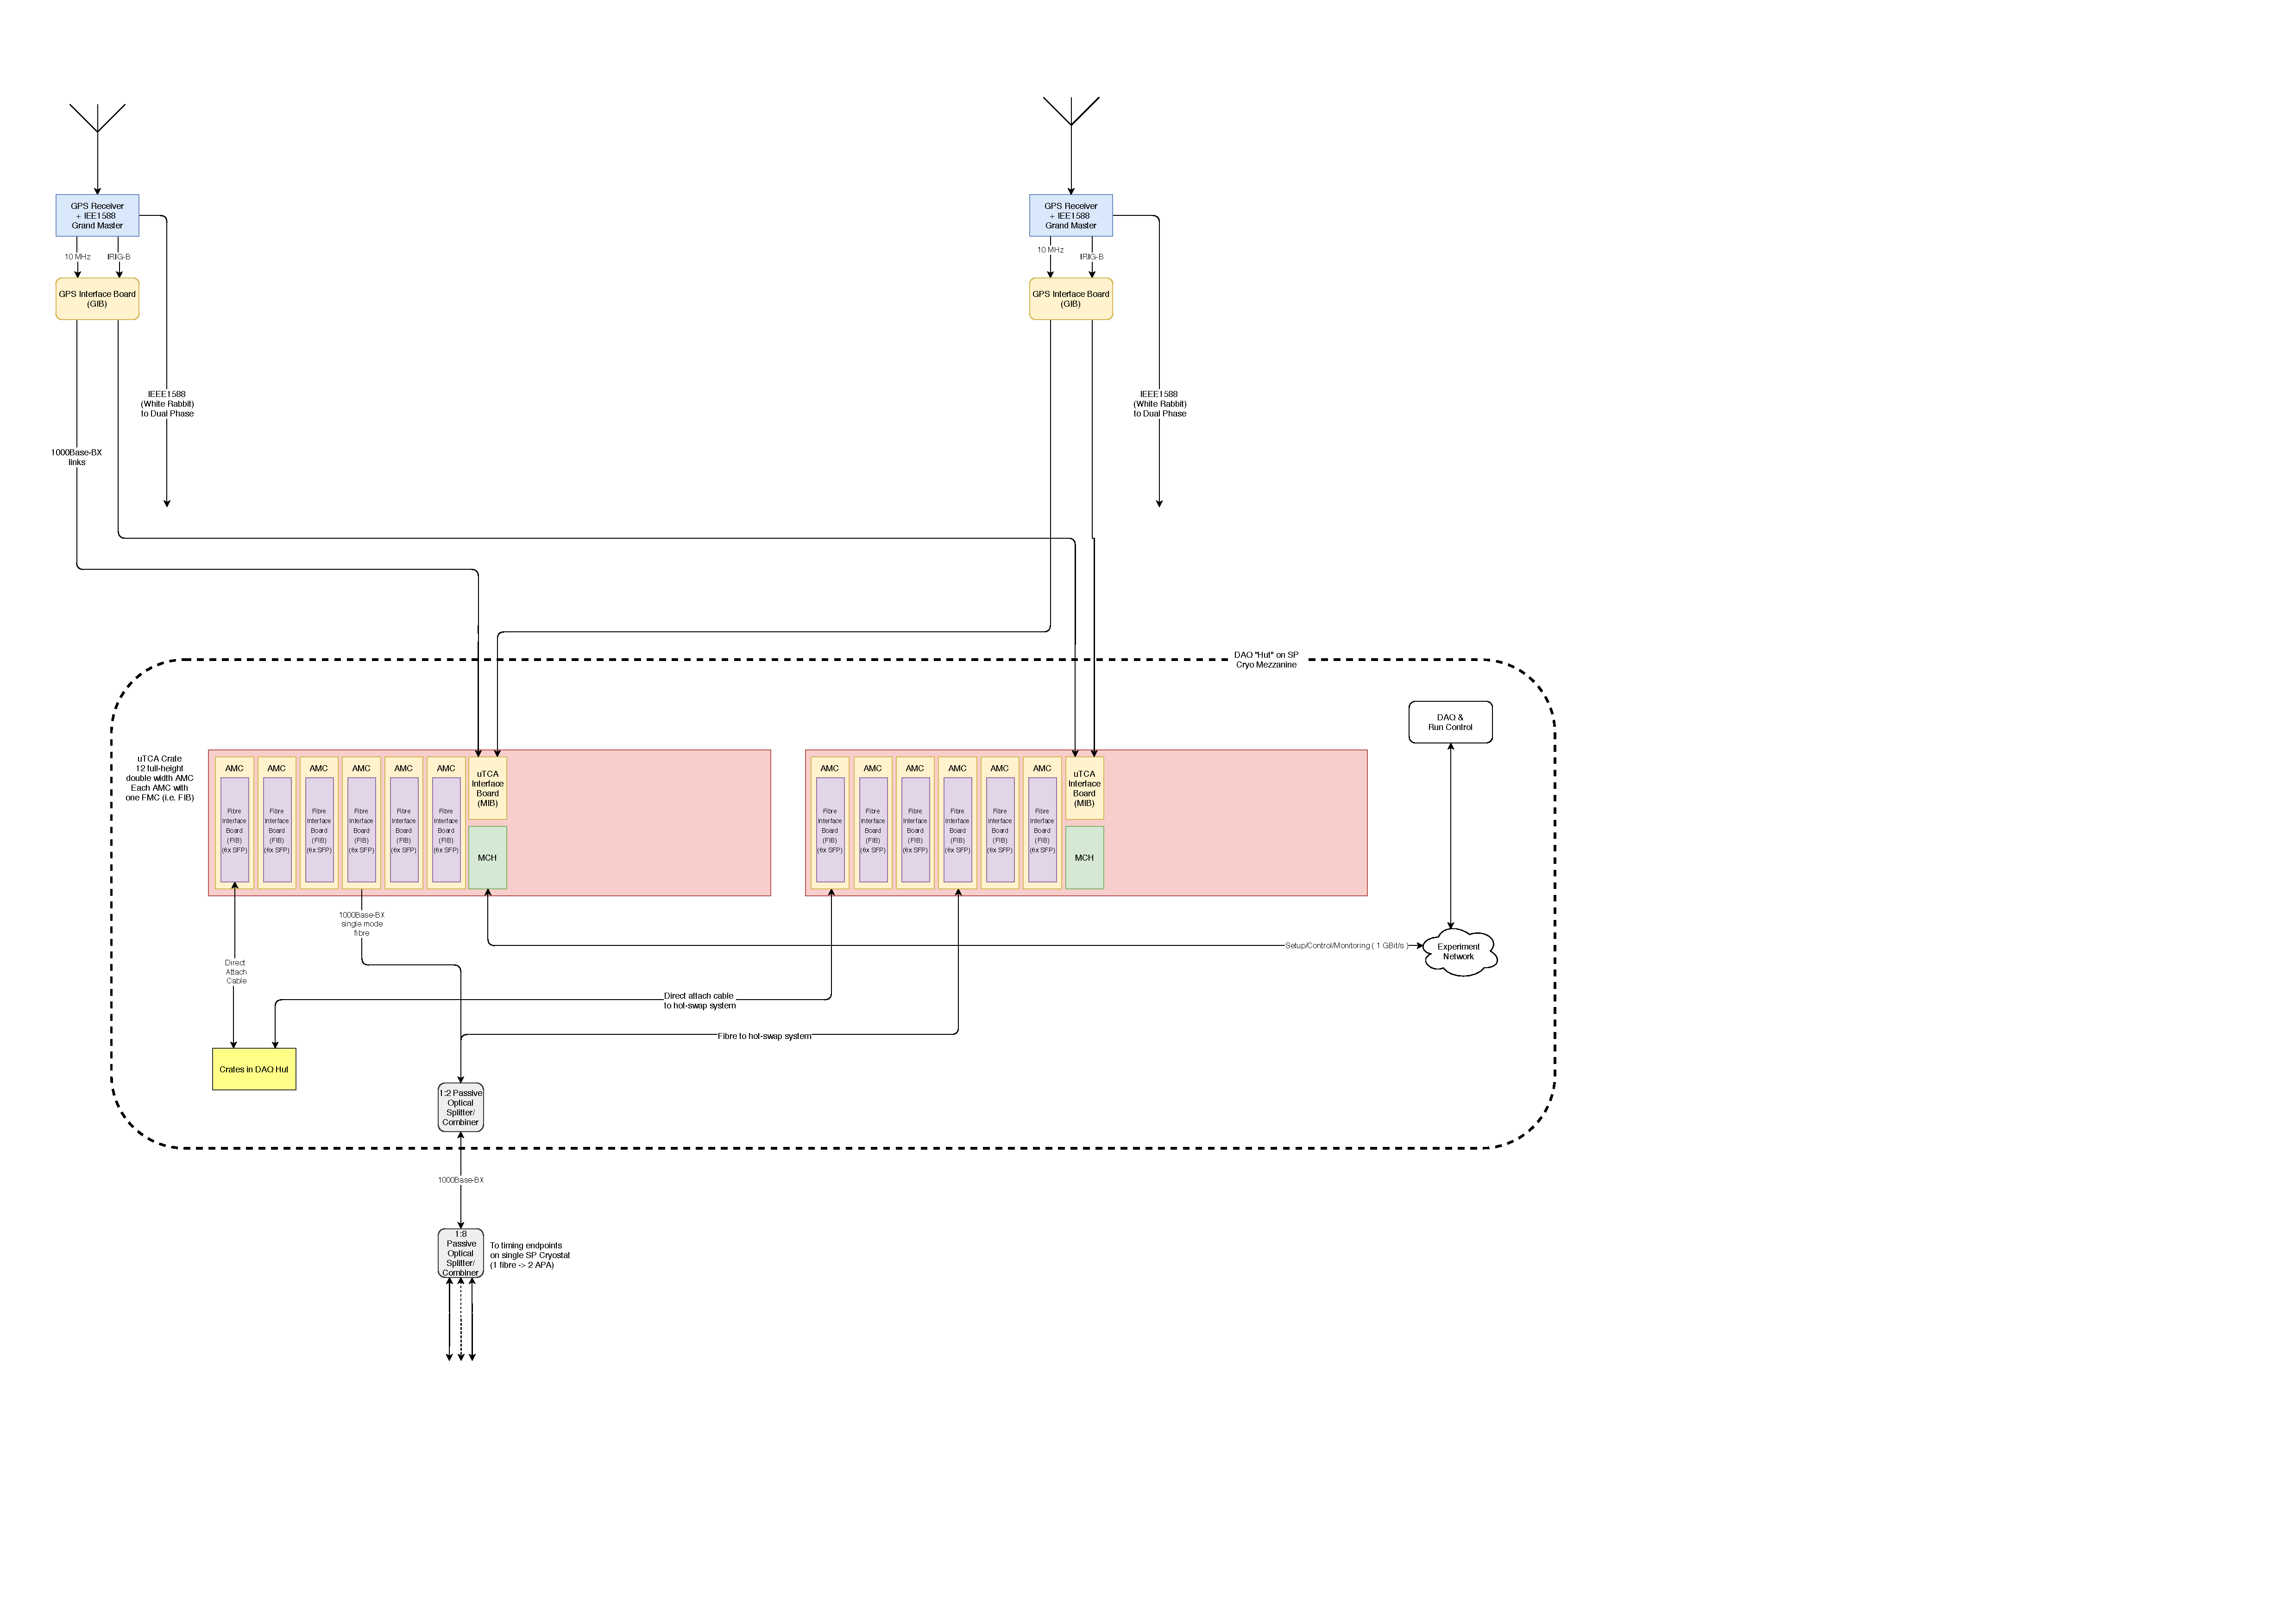
\includegraphics[width=\textwidth]{DUNE_SP_Timing_DAQ_on_CryoM_GPS_In_CUC_16mar20.pdf}
\caption{Illustration of the components in the \dword{spdts}.}
\label{fig:daq-readout-timing}
\end{figure}

In order to provide redundancy, and also the ability to easily detect
issues with the timing path, two independent GPS systems, i.e. GPS receiver+\dword{gib}, are used. One with an antenna at the head of the Yates Shaft, the other with an
antenna at the head of the Ross Shaft. The two independent timing
paths are brought to each \dword{detmodule} cavern, where they both feed two independent redundant \dword{utca} crates, each equipped with a \dword{mib} and a set of six \dwords{amc}+\dwords{fib}. Using 2:1 fibre combiner/splitters, one \dword{spdts} unit can be left as a hot spare while the
other is active. This also allows testing of new firmware and software
during commissioning without the risk of losing the \dword{spdts} if a bug is
introduced.

\subsection{GPS receiver}
In order to meet the synchronisation requirements outlined in section \ref{sec:intro}, the \dword{dts} needs a stable timing reference from which to generate the \dword{sp} and \dword{dp} clocks. The reference clock must have both excellent short and long term stability. Such a clock can be provided by a \dword{gpsdo}, which works by locking the output of a high quality quartz crystal or rubidium oscillator to a GPS signal. A GPSDO combines the long term stability of a GPS signal, with the short term stability of an oscillator.

A GPS signal can also be used to provide an absolute time reference, as GPS time is locked to \dword{utc}. The time from the GPS signal will be used to initialise and cross-check the timestamp provided by the \dword{dts}.

The \dword{dts} is envisaged to use the SecureSync Time and Frequency Synchronization System \cite{secure_sync_datasheet} as its GPS receiver. The SecureSync system provides a \SI{10}{\MHz} clock generated by a GPS disciplined \dword{oxco}. The GPS time signal will be output by a dedicated module \cite{secure_sync_modules} using an IRIG time code \cite{irig}. IRIG time codes are a standardised format of transmitting timing information. The \SI{10}{\MHz} clock and \dword{irig} data stream will be transmitted to the \dword{gib} using BNC connections.

The GPS receiver will also host a module \cite{secure_sync_modules}, which will output an IEEE 1588-2008 \cite{ieee_1588_2008} timing signal to the \dword{dp} \dword{wr} \cite{wr_ohwr} timing network.

\subsection{GIB}
The \dword{gib} receives the \SI{10}{\MHz} reference from the GPS receiver, and uses it to generate the \SI{62.5}{\MHz} \dword{spdts} clock. The clock is generated using an SI5344 chip, enabling the highest level of jitter performance. The IRIG time code is decoded by the \dword{gib} FPGA, and used to initialise the \dword{spdts} timestamp. After initialisation, the \dword{spdts} timestamp is maintained by the \dword{gib} firmware, where it is continuously updated using the \SI{62.5}{\MHz} clock. The firmware also continuously monitors, and records, the relationship between \dword{utc} and the \dword{spdts} timestamp.

Synchronisation messages, containing the \dword{spdts} timestamp, are generated by the \dword{gib} and transmitted to the \dwords{mib} using the \dword{spdts} protocol over single mode optical fibres. Before transmission, the 8b/10b encoded \dword{spdts} data stream is re-clocked using a high-speed D flip-flop running at \SI{312.5}{\MHz}. The \SI{312.5}{\MHz} clock is derived from the same reference as the \dword{spdts} clock, and is generated by the same IC.

The optical fibre link to the \dword{mib} is bi-directional, where the outgoing and incoming signals are transmitted using different wavelengths, transmitting happens at \SI{1310}{nm}, whereas receiving is at \SI{1550}{nm}. The return data path will be used to measure the time delay between the \dword{gib} and the \dword{mib}, allowing the \dword{spdts} to compensate for it. The logical layout of the \dword{gib} is shown in figure \ref{fig:gib_layout}.

\begin{figure}[h]
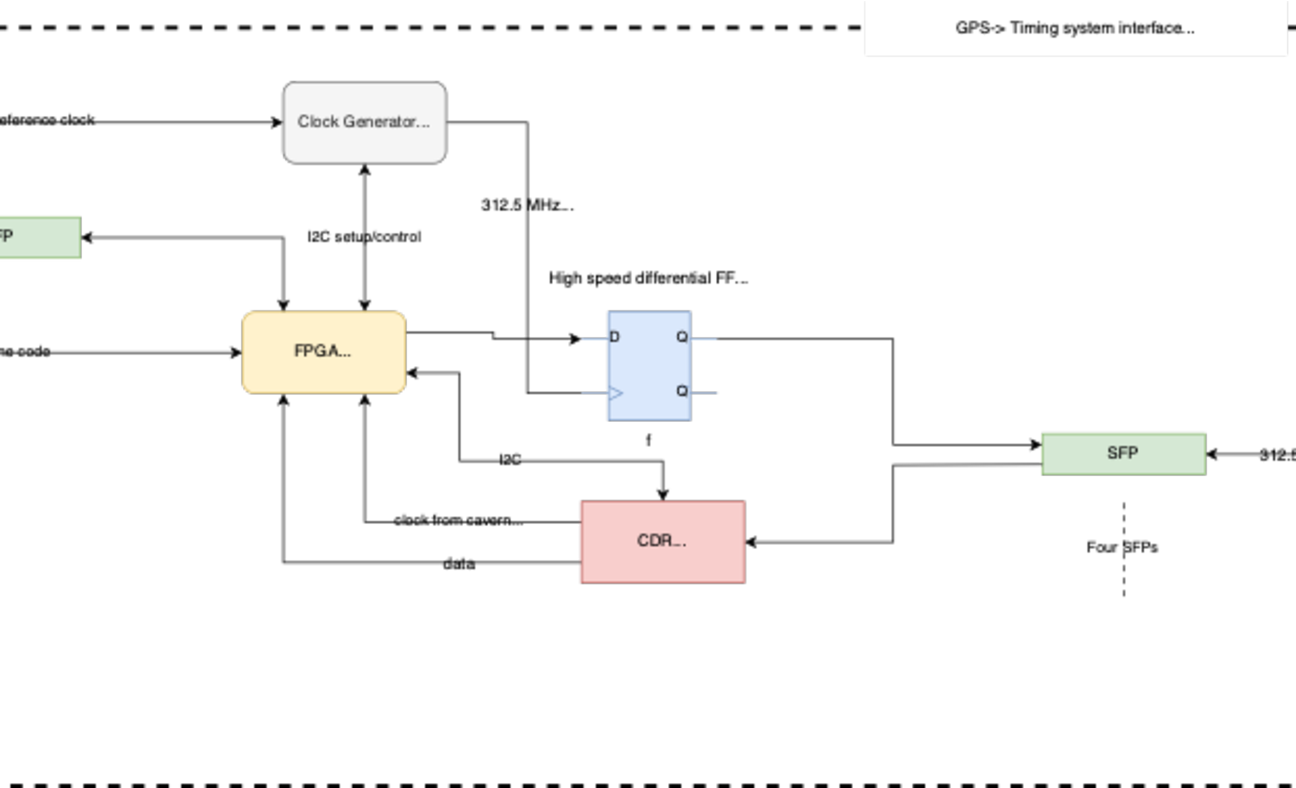
\includegraphics[width=\textwidth]{gib_layout.pdf}
\caption{Illustration of the components in the \dword{gib}.}
\label{fig:gib_layout}
\end{figure}

Control and management of the \dword{gib} and GPS receiver will be done using a gigabit ethernet.
\subsection{MIB}
The \dword{mib} receives the \dword{spdts} data stream from the \dword{gib} and decodes it into separate clock and data signals using a commercial \dword{cdr} IC. The recovered clock is fed into an SI5344 chip to regenerate a low jitter \SI{312.5}{\MHz} clock. The regenerated clock is fanned out to the six \dwords{amc} over the \dword{utca} backplane using a clock fan-out chip. The recovered data is sent directly into the \dword{mib} FPGA. The upstream data stream, i.e. from the \dword{mib} to the \dword{gib}, is re-clocked using the low jitter \SI{312.5}{\MHz} clock, before being sent out over the optical fibre.

The \dword{utca} backplane provides three point-to-point differential connections between the \dword{mib} and each \dword{amc}. One of the links is used to fan out the \SI{312.5}{\MHz} clock to the \dwords{amc}. Another one is used to transmit \dword{spdts} timing data to each \dword{amc}. The third line serves as a return data path, from each \dword{amc} back to the \dword{mib}. An illustration of the different \dword{mib} components is shown in figure \ref{fig:mib_layout}.

\begin{figure}[h]
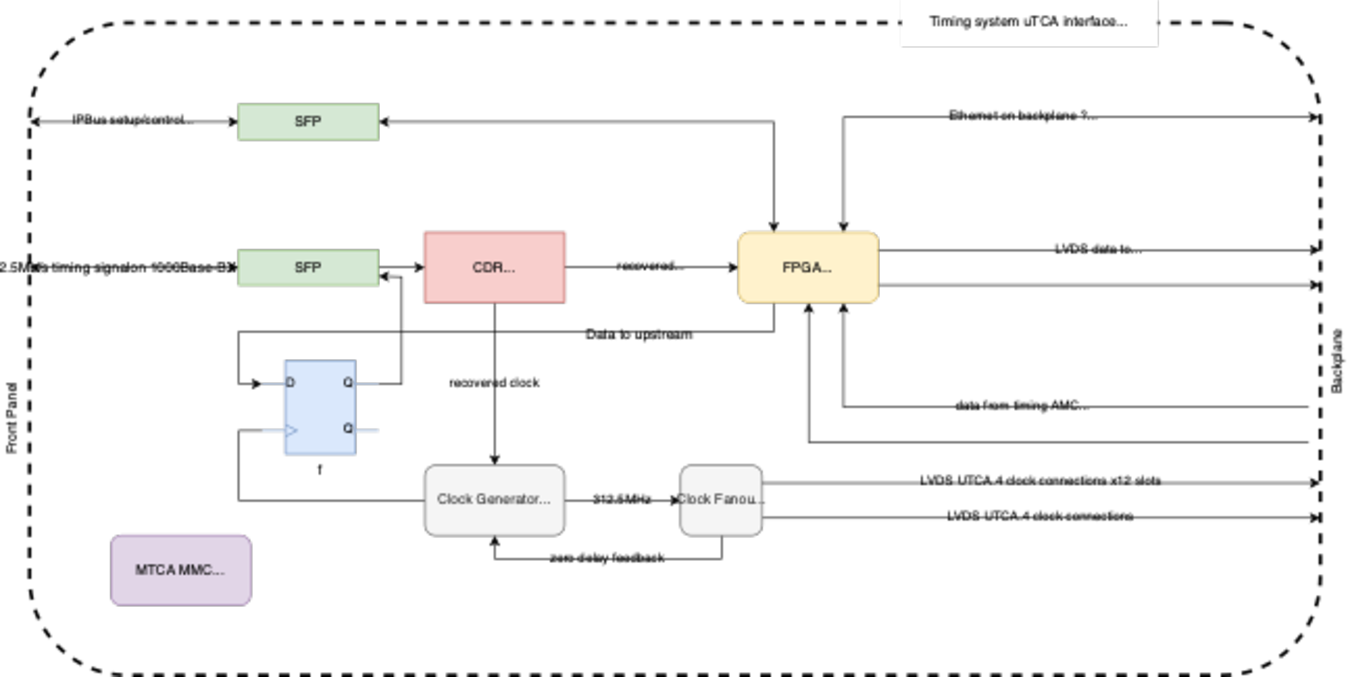
\includegraphics[width=\textwidth]{mib_layout.pdf}
\caption{Illustration of the components in the \dword{mib}.}
\label{fig:mib_layout}
\end{figure}

The \dword{mib} has the following functions:

\begin{itemize}
	\item Reception of external timing and trigger signals
	\item Logging and time-stamping of signals received, distributed or throttled, and transmission to DAQ
	\item Serialisation of timing commands and transmission to the timing network
	\item Phase measurement of incoming timing signals from slaves, i.e. \dwords{fib} and timing endpoints, allowing phase adjustment under software control
	\item Transmission of arbitrary commands and control data under software control
\end{itemize}

The reception of external signals will be achieved using the return data path from a dedicated timing endpoint connected to a \dword{fib}. The external signals will be timestamped onto \dword{spdts} time domain by the dedicated endpoint. The external signal \dword{spdts} message will then be sent from the endpoint, to the \dword{mib}, via a \dword{fib}. Depending on the type of external signal message, the \dword{mib} may redistribute it to all timing endpoints, or take another action. 
As well as timestamping external signals onto the \dword{spdts} time domain, the \dword{mib} will do the same for \dword{wr} synchronization signals from the \dword{dp} \dword{detmodule}. Reciprocally, \dword{spdts} synchronization signals will be timestamped onto the \dword{dp} clock domain. This allows the timing in the \dword{sp} and \dword{dp} \dwords{detmodule} to be
aligned. A similar scheme is used to relate the \dword{spdts} timing domain to the beam instrumentation \dword{wr} time domain.

To allow timing commands to take effect at all endpoints simultaneously, the delay between the command source, i.e.\ \dword{mib}, and each endpoint, must be measured and compensated for. To achieve this, both the \dword{mib}-\dword{fib}, and \dword{fib}-endpoint delays, must be ascertained.

The interface to the DUNE DAQ and \dword{ccm} systems will be implemented over gigabit ethernet. The \dword{utca} backplane will provide an ethernet connection between the \dword{mib} and the \dword{mch}, which in this case, acts as an
ethernet switch.

\subsection{FIB and its carrier}
The \dword{fib}, together with its carrier (an \dword{amc}), act as an active fanout for the \dword{spdts} clock and data stream. The clock delivered to the \dword{amc} over the \dword{utca} backplane is routed to the \dword{fib}, where it is fed into a SI5344 IC, generating a low jitter version of the clock. The incoming data is routed to the \dword{amc} FPGA, where it is decoded and also fanned out to the eight \dword{sfp} modules on the \dword{fib}. As before, the \dword{spdts} data is re-clocked on the low jitter version of the \SI{312.5}{\MHz} clock using a D-type flip-flop, before it is sent out.

The \dword{fib} is also used to arbitrate which of the eight \dword{sfp} modules is sending data upstream back to the \dword{mib}. This is achieved via an 8:1 differential multiplexer controlled by the \dword{amc} FPGA. \textcolor{red}{Is this true? how does this affect the external signals endpoint?} The output of each of the \dword{sfp} modules is connected to an 1:8 passive optical splitter/combiner, allowing each \dword{sfp} to service two \dwords{apa}, assuming four timing endpoints per \dword{apa}. The fact that multiple endpoints are connected to one \dword{sfp} means that only one endpoint can send \dword{spdts} data at a time. The endpoint receiving the external triggers will not be connected to an optical splitter/combiner. A block diagram of the components of the \dword{fib} and its carrier is shown in figure \ref{fig:fib_and_carrier_layout}.

\begin{figure}[h]
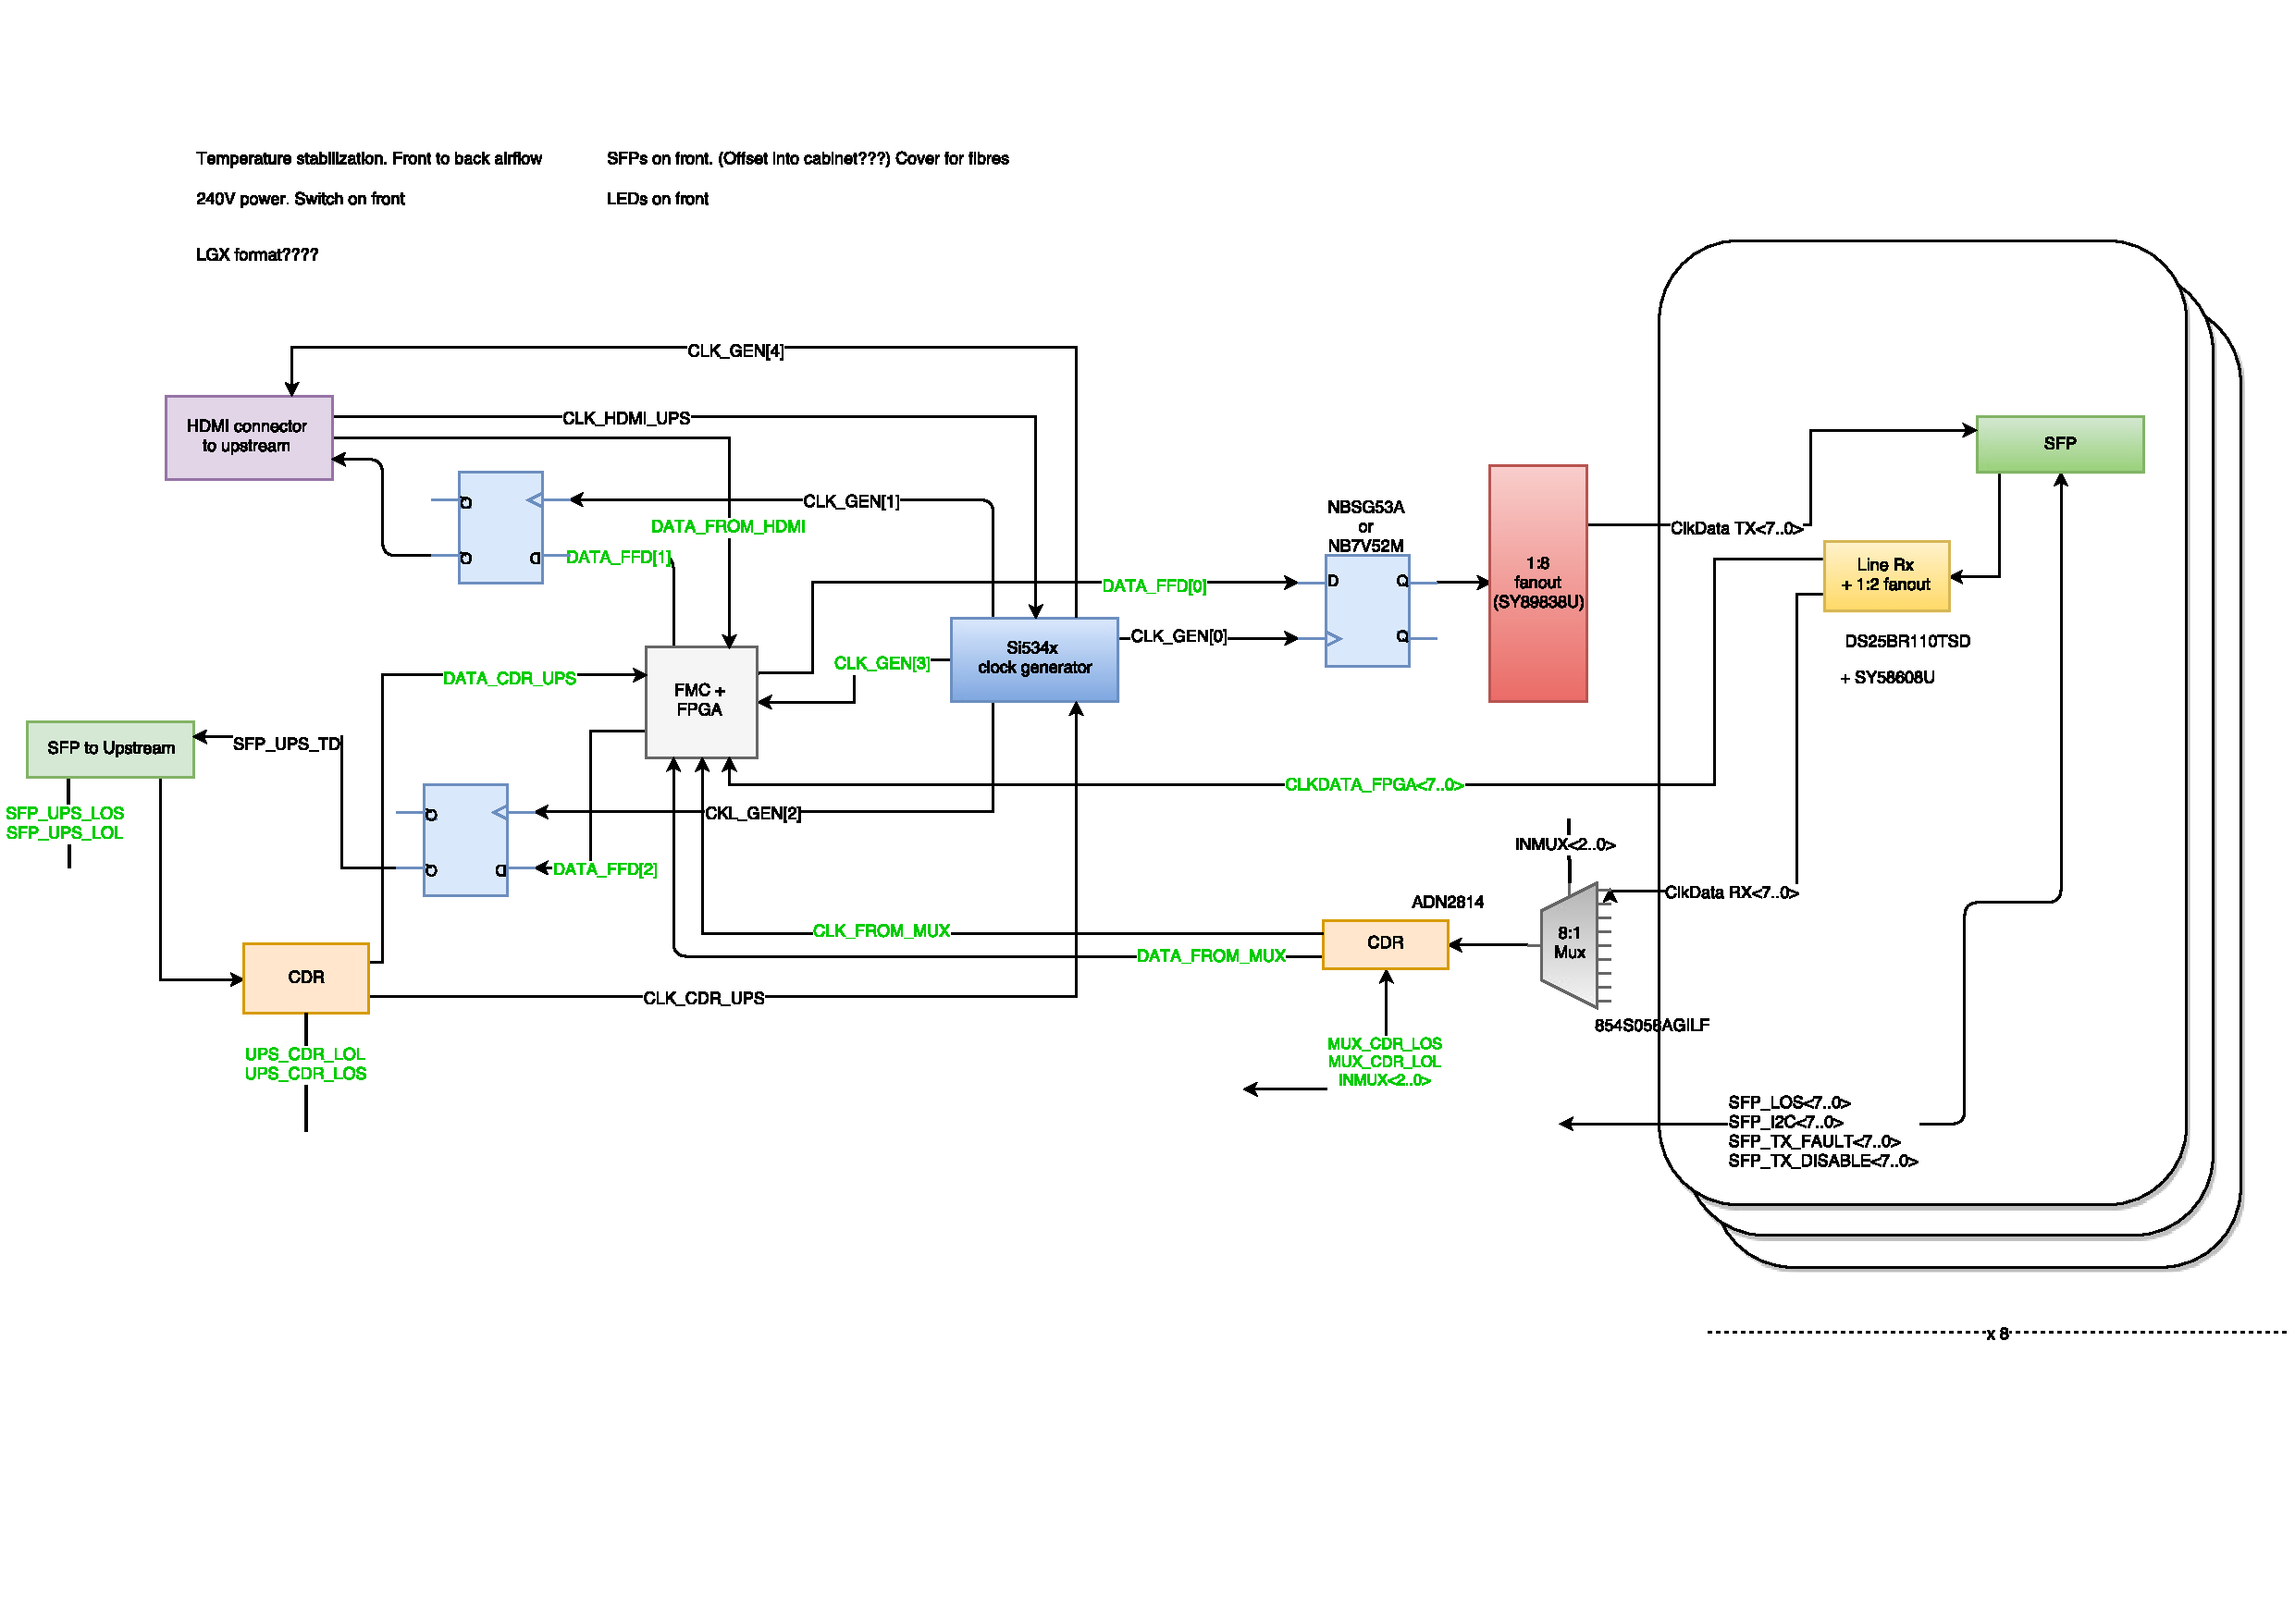
\includegraphics[width=\textwidth]{protoDUNE_timing_system_active_fanout.pdf}
\caption{An illustration of the \dword{fib} and its carrier. \textcolor{red}{This ia a diagram of the ProtoDUNE-SP I fanout unit, replace with actual diagram.}}
\label{fig:fib_and_carrier_layout}
\end{figure}

The \dword{fib} carrier is envisaged to be off-the-self \dword{amc}. The ohwr.org hosted \dword{afc} design \cite{amc_ohwr}, is currently being evaluated as a potential candidate.

The \dword{fib} will be a development of the existing timing \dword{fmc} used in ProtoDUNE-SP I. A photo of the existing timing FMC, and a mock-up of the \dword{fib} are shown in figures \ref{fig:timing_fmc} and \ref{fig:fib_mockup} respectively.

\begin{figure}[h]
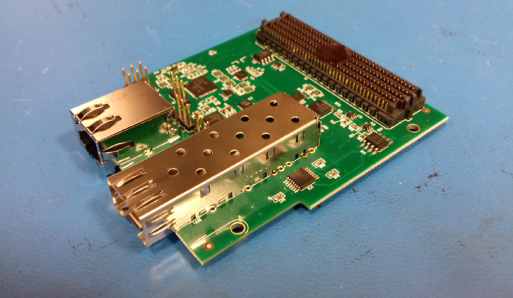
\includegraphics[width=\textwidth]{timing_fmc.pdf}
\caption{A photo of the existing timing FMC.}
\label{fig:timing_fmc}
\end{figure}

\begin{figure}[h]
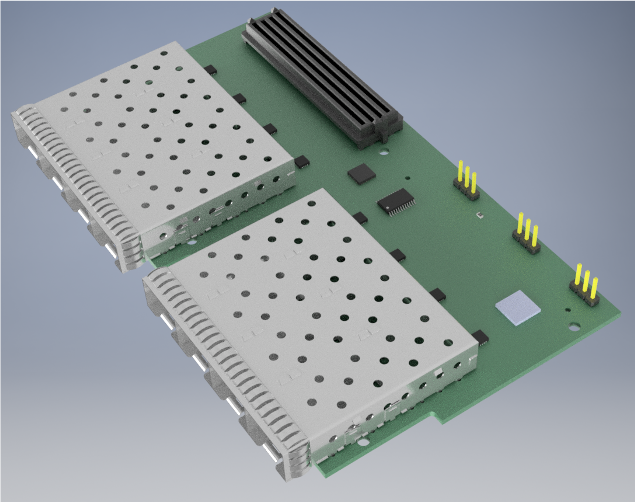
\includegraphics[width=\textwidth]{fib_mockup.png}
\caption{A mock-up of the \dword{fib}.}
\label{fig:fib_mockup}
\end{figure}

Monitoring and control of each \dword{amc} and its \dword{fib} will be done over gigabit ethernet. Similarly as before, the \dword{utca} backplane provides an ethernet connection between each \dword{amc} and the \dword{mch}, which will act as an ethernet switch.

\subsection{Endpoint}
Endpoints decode the timing signal into separate clock and data
signals using a \dword{cdr} IC, which in turn feeds a low-bandwidth PLL for applications requiring a very low jitter local clock. A common firmware block is used to decode the timing protocol, which is incorporated into the overall
firmware design for the receiving FPGA in each DAQ component. This
`block provides a cycle counter, several independent trigger, calibration and 
synchronisation signals, and a general-purpose packet data output to each endpoint. The cycle counter may be used further to generate low-frequency timing signals for further propagation, e.g. the \SI{2}{\MHz} sampling signal for the cold ADCs.
\subsection{Redundancy}
The extremely high uptime requirements of the DUNE experiment translate into similarly high uptime requirements on the timing system. The uptime requirements on the timing system may even exceed those of the overall experiment due to the fact that the timing system is an essential part of the experiment infrastructure, and no system can operate without it.

To facilitate the uptime requirements, the timing system has been designed to include two complete and independent timing chains, where the whole or a part of one system is active, and the other one acts as hot spare.

There are two GPS antennae, one on top of the Yates shaft and another on top of the Ross shaft. Each antennae feeds a GPS receiver and a \dword{gib}, producing two independent \dword{spdts} clocks and timestamps. Cross-referencing the two independent signals, potentially against a third signal, e.g. a rubidium oscillator, allows for any drifts or other issues in one of the \dword{spdts} timing streams to be detected. At any one time, only one of the \dword{spdts} clock and timestamp are actively used.

The two \dword{spdts} timing streams are both fed into two \dword{utca} crates. There is one set of two \dword{utca} crates per \dword{spmod}. Each crate is populated with the full timing \dword{utca} payload, i.e. a \dword{mib}, \dword{mch}, and six \dwords{amc} and \dwords{fib}. The output of the two crates is brought together into a passive optical splitter/combiner, allowing the swapping of active crates without physical intervention.

The design also allows, both crates to be partially active. This may be useful in a scenario, where a \dword{fib} in the active crates becomes faulty, and the recovery action would be to enable the equivalent \dword{fib} in the redundant crate. This would isolate the disruption of the timing signal only to the endpoints supplied by the faulty \dword{fib}, rather than the whole \dword{spmod}. It is also possible to use just a single \dword{sfp} module of the redundant crate, minimising disruption to the DUNE data-taking even further.

The arbitration of which \dword{spdts} timing stream and physical hardware is providing the timing for the \dword{spmod} will be done by the DUNE \dword{ccm}. The \dword{ccm} system is natural candidate for this role, as it has high-level overview of the whole DUNE detector, including the timing system. The CCM may initiate a hot-swap action, however the responsibility for the actual implementation and execution of the swap mechanism lies in the domain of the timing system.

\subsection{Internal interfaces}
This section seeks to describe the physical \textcolor{red}{(and later software+firmware?)} interfaces between the different components of the \dword{spdts} and \dword{dpdts}. 

\subsubsection{GPS receiver-\dword{dpdts}}
The GPS receiver houses a IEEE 1588 (PTP) grandmaster and a source of IRIG time codes. The PTP grandmaster provides a timing signal for the \dword{dp} \dword{wr} timing network. The \dword{dpmod} uses the \dword{wr} implementation of the IEEE 1588-2008 timing distribution standard. The components that distribute the timing signals are included in the scope of the \dword{dp} readout electronics and are not described here. The interface between the \dword{dts} and the \dword{dp} readout electronics is by means of 1000Base-BX \dword{sfp} coupled by single mode fibre. There will be two fibres carrying IEEE 1588-2008 timing signals supplied to the \dword{dp} readout electronics, one from each of the two GPS receivers.

\subsubsection{GPS receiver-\dword{gib}}
There are two distinct hardware interfaces between the GPS receiver and the \dword{gib}. One delivering the \SI{10}{\MHz} reference clock from the GPS receiver to the \dword{gib}, the other transmitting \dword{irig} time code, containing the \dword{utc} timestamp. Both interfaces are realised using coaxial cables and BNC connectors.

The two physical units are envisaged to be close to each physically, either in the same or adjacent computing racks. This means that the length of the cables connecting the two devices will not exceed a few metres.

\subsubsection{\dword{gib}-\dword{mib}}
Each \dword{gib} will need connect to two \dwords{mib} per \dword{spmod}, where each connection will use a single mode fibre. The \dword{gib} and \dword{mib} will have \dword{sfp} cages, which will host 1000Base-BX-20 \dword{sfp} transceivers which transmit at 1310 nm and receive on 1550 nm. Since the \dword{gib} will be on the surface, and the \dword{mib} underground, the optical cables will be several km long.

\subsubsection{\dword{mib}-\dword{amc}}
The \dword{mib}, will sit in the primary \dword{mch} slot of the \utca crate, and will use three differential point-to-point lines to transmit and receive timing data from the six \dwords{amc}. The connections are provided by the \dword{utca} backplane. The FCLKA and TCLKA lines from the \dword{mib} are routed to CLK1 and CLK2 on each \dwords{amc}. These lines will be used to transmit the \dword{spdts} clock and data stream respectively. CLK3 from the \dwords{amc} is routed to TCLKB on the \dword{mib}. Two differential lines are used to establish a 1000BASE-X ethernet connection between the \dwords{amc} and the actual \dword{mch}, residing in the secondary \dword{mch} slot. An illustration of the connections inside the \dword{utca} is shown in figure \ref{fig:mib_utca_connections}.

\begin{figure}[h]
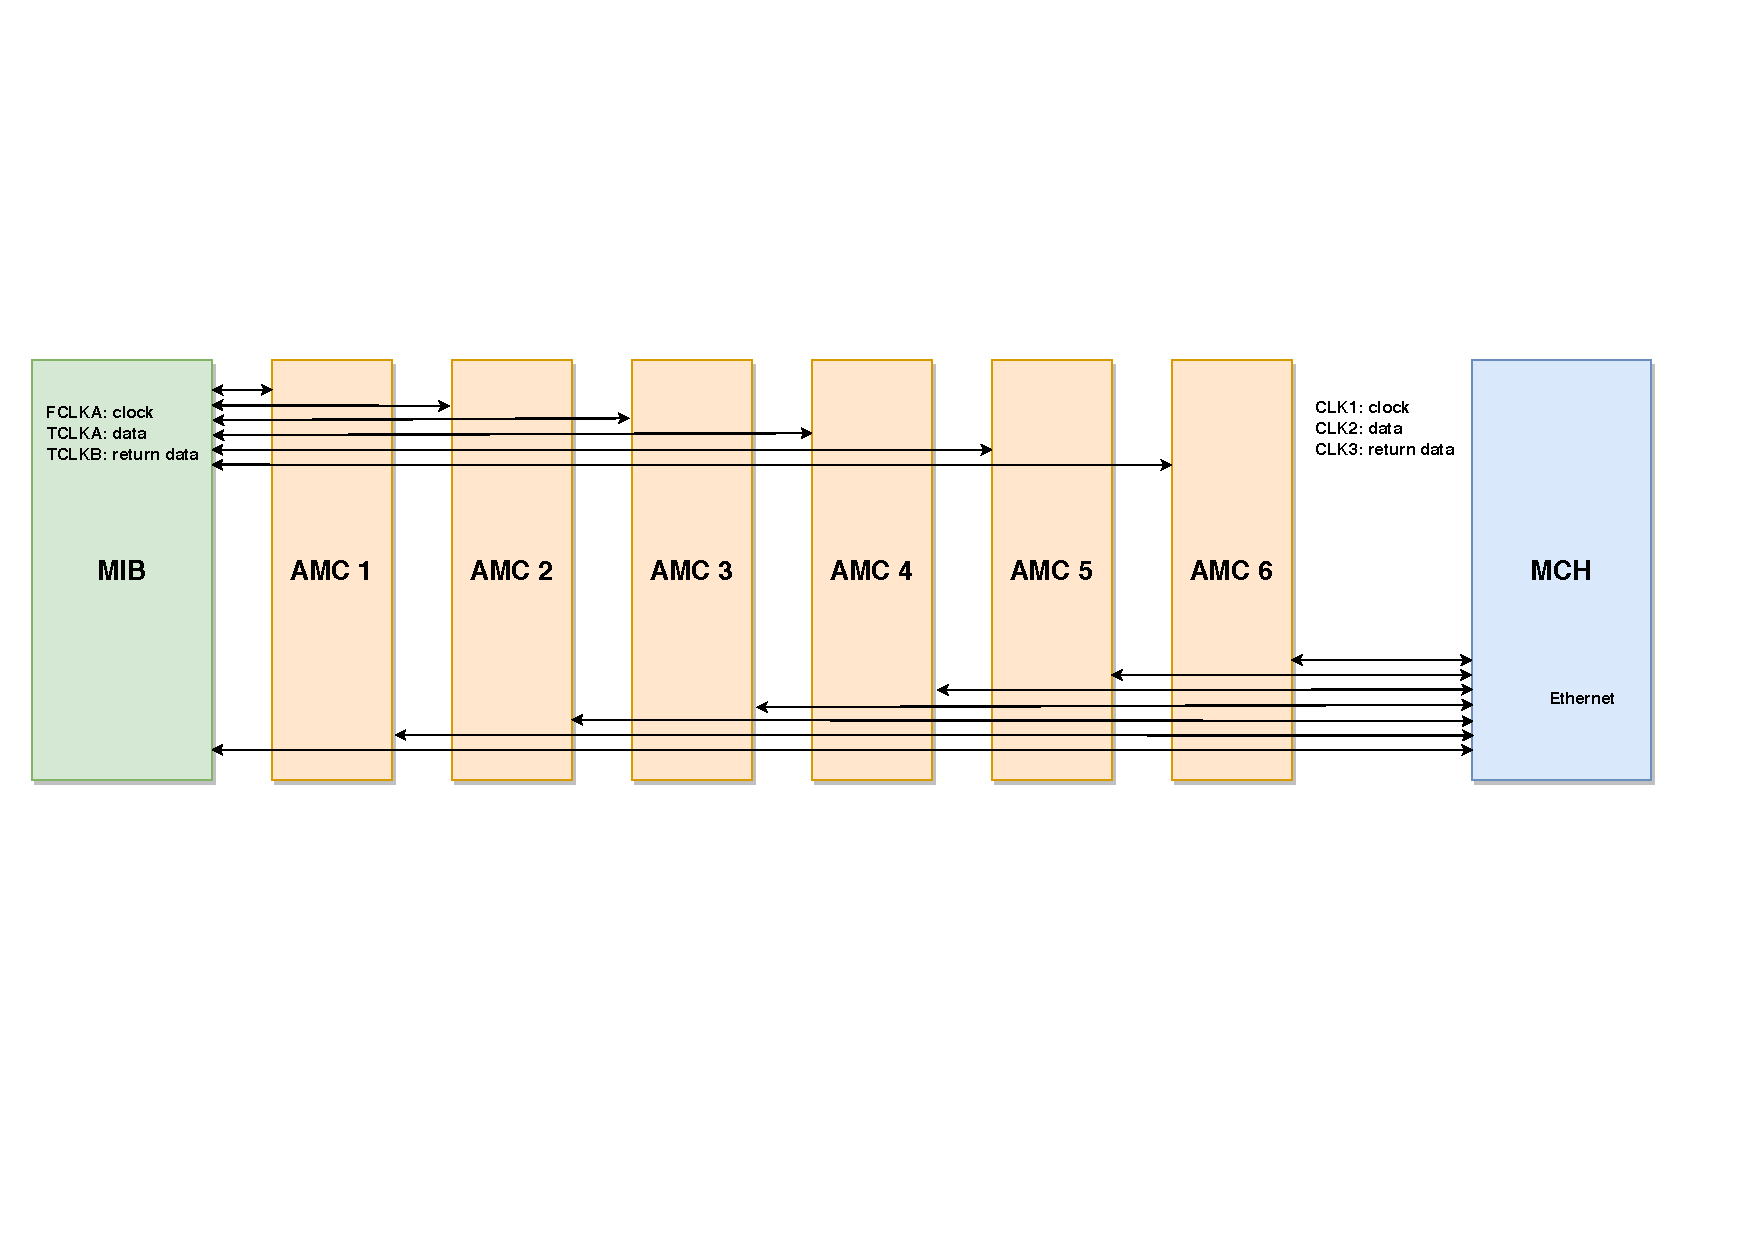
\includegraphics[width=\textwidth]{mib_utca_connections.pdf}
\caption{An illustration of the connections between \dword{mib} and \dwords{amc} inside the \dword{utca} crate.}
\label{fig:mib_utca_connections}
\end{figure}

\subsubsection{\dword{amc}-\dword{fib}}
The connection between the \dword{fib}, which is an \dword{fmc}, and its \dword{amc} carrier will be achieved using a \dword{hpc} \dword{fmc} connector. The \dword{afc} has two such connectors, however since the \dword{fib} is a single double-width \dword{fmc}, only one will be used.
\subsubsection{\dword{fib}-endpoint}
The output of the 48 ($6\times8$) \dword{sfp} modules from the two \dword{utca} crates will be brought together into a 2:1 passsive optical combiner/splitter. This configuration allows the switching of operation between the two crates to happen without physical intervention. The output of the 2:1 optical combiner will be fed into a 1:8 splitter/combiner, which is used to fan out the \dword{spdts} timing stream to the endpoints. The optical connections will use single-mode fibres, and 1000Base-BX-20 \dword{sfp} transceivers, transmitting at 1310 nm and receiving on 1550 nm. Due to the use of the optical splitter to fan out the timing signal, only one endpoint at a time can transmit a return signal.
\subsection{\dword{spdts} protocol}
\textcolor{red}{description of the spdts protocol goes here}
\section{Design and system validation}
The development and validation of the \dword{dts} is based around iterative incremental model, where the functionality of the system is built up step-by-step. As per the overall DUNE development strategy, each system or technology  which will be used in the eventual DUNE \dword{fd} must first be demonstrated to be fit for purpose at the ProtoDUNE experiments at CERN. The timing system is no different, and has fully embraced this ethos. Two distinct \dword{spdts} prototypes will be used for the two phases of the ProtoDUNE SP experiment. The use of the \dword{spdts} at the ProtoDUNE experiments will be especially useful in validating the operational requirements, external system interfaces, and long-term stability of the system. The validation of the \dword{spdts} system will also heavily rely on test and measurements performed in a laboratory environment, e.g. alignment of timing endpoints to within \SI{1}{ns}. 

\subsection{Tests at ProtoDUNE-SP I}
A prototype of the \dword{spdts} was developed and successfully used to synchronise the components of ProtoDUNE SP I. The system uses an AIDA 2020 TLU as a master unit, which receives external signals from the trigger system and SPS accelerator, as well as a high-quality \SI{10}{\MHz} reference, which is used to generate the ProtoDUNE SP I \SI{50}{\MHz} clock. The master unit also multiplexes synchronization and trigger commands, along with arbitrary command
sequences generated by software, into a single encoded data stream. The timing data stream is fanned out to the endpoints via the means of an active fanout module and single-mode fibres. At each endpoint, a commercial \dword{cdr} device is used to recover separate clock and data signal from the data stream, which are used to synchronise the endpoint.

The system operated successfully for the duration of the data-taking and has demonstrated the following functionalities:

\begin{itemize}
    \item generation and distribution of a stable master clock to DAQ components
    \item timestamping of external signals onto the ProtoDUNE SP I time domain
    \item distribution of synchronisation, trigger and calibration commands to the DAQ system.
\end{itemize}

These functionalities form a core part of the expected role of the \dword{dts}, however certain other key aspects of the system were not tested at ProtoDUNE SP I. Some of these include:

\begin{itemize}
    \item GPS interface and IRIG decoding
    \item Synchronisation with UTC
    \item Synchronisation between endpoints
    \item \dword{utca} fanout hardware.
\end{itemize}

The issues listed above will be addressed by the prototype developed for ProtoDUNE SP II, as well as prototype testing in a laboratory.

\subsection{Tests at ProtoDUNE-SP II}
The ProtoDUNE-SP I timing system demonstrated several key functions of the eventual \dword{spdts}, however the hardware used to construct the prototype is not aligned with that of the actual DUNE \dword{spdts}. This issue be remedied by the ProtoDUNE-SP II prototype, which will use the full chain hardware components described in section \ref{sec:system_design}, i.e. from GPS receiver to timing endpoint. This second prototype will also be used to test synchronisation between endpoints and UTC. The validation of these requirements will be done both at ProtoDUNE SP II and in the laboratory. The frequency of the system clock will be increased to the expected \dword{spdts} value of \SI{62.5}{\MHz}.

Another advantage of deploying timing system prototypes at the ProtoDUNE experiments is that it allows the assessment of the long-term stability of the system, and associated operational challenges. This type of long-term operation feeds directly into the validation of the uptime requirements of the final \dword{dts}.

\subsection{Tests in laboratory}
For ProtoDUNE SP II, it is not envisaged that a fully redundant system will be deployed, however the functionalities associated with having two independent timing chains must still be developed and tested. Most of this work will be carried out in a laboratory setting, with a representative setup of the \dword{dts}. Laboratory tests will also be needed to carry out disruptive tests, such as endpoint or system wide fault recovery and firmware development.

\section{Commissioning}
The \dword{dts} will be one of the first DAQ components installed, so that timing and synchronization signals are available the other components of the DAQ as soon as they start to be installed. Early in the construction project \dword{spts} ``development kits'' will be made available. The kits will include the hardware and software needed to produce \dword{spts} timing signal. This will allow the teams developing the DUNE readout systems to integrate with the \dword{spts} early in the development process. Hardware and software will also be available for use in vertical slice tests and the \dword{itf}. 

\printglossary
\printbibliography

\end{document}
